% Put the project details here
\section{PROJECT DETAILS}

    International School Manila handles the process of Sponsorship Billing and Letter of Guarantee coverage in PowerSchool (SIS), Student Charging Portal, NetSuite (ERP), and Online Billing System. The deployed pilot web application added a Sponsor Management layer to the web application, which is used to centralize sponsor profiles, contacts, addresses, LoG rules, and to evaluate at the point of charge entry. This design choice makes the decision of Covered / Not Covered more accurate, less rework and more auditable in the ERP and statement layer. A controlled pilot application is available at \url{http://ismsponsor.azurewebsites.net/} for the running version. % FORMAT HIGHLIGHT: URL formatting

    %Streamline Overview
    \begin{figure}[H]
    \begin{center}
        \vspace{2ex}
        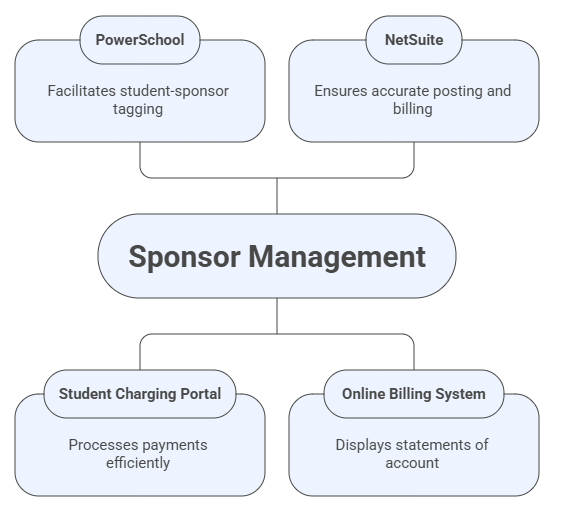
\includegraphics[width=300pt]{images/streamline.png}
                \caption{Streamlining Sponsor Management}
                \label{fig:Streamlining Sponsor Management}
    \end{center}
    \end{figure}
    
    As shown in Figure~\ref{fig:Streamlining Sponsor Management}, the proposed Sponsor Management layer is the common point of reference for PowerSchool, Student Charging Portal, NetSuite and Online Billing System. The figure is provided to illustrate the centralization of sponsor records and the rules for coverage of LoG before deciding on billings and sending to finance and statement systems.
    
    PowerSchool is used for sponsor tagging of students, NetSuite is the posting/billing ledger, the Sponsor Management layer holds all sponsor information and LoG rules, the Student Charging Portal is used for charge entry and coverage evaluation, and the Online Billing System publishes statements showing the final Bill-To and allocations.
    
    \subsection{Overview}
    
    This work resulted in a deployed pilot web application, at \url{http://ismsponsor.azurewebsites.net/}, where sponsors will be able to use self-service functions to manage their information (name, TIN, addresses, multiple contacts), obtain a list of LoG entries for each student per school year, and create or edit LoG entries via a guided modal form with status tracking.

        %Context Diagram
        \begin{figure}[H]
        \begin{center}
            \vspace{2ex}
            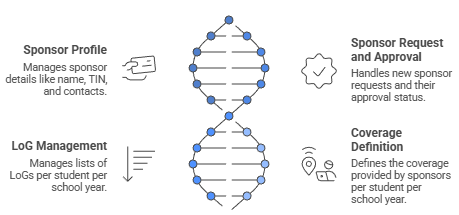
\includegraphics[width=400pt]{images/Application Features.png}
                \caption{Application Features}
                \label{fig:Application Features}
        \end{center}
        \end{figure}
    
    The main features of the pilot are described in Figure~\ref{fig:Application Features}, such as managing the sponsor profile, managing LoG, defining the coverage, handling sponsor requests, reporting support, etc. The figure is added to relate the introduced modules to the request to have a constant sponsor billing governance during operation. The system offers real-time calculation of preview for coverage on the Student Charging Portal and generates a decision with reason codes for operators.

    \subsection{Project Framework}
    
    Development was done in a DevOps manner with small tested releases to provide the ISM Sponsor Management and LoG Coverage Integration System. Requirements and integration mapping was validated initially, followed by development of features with automated builds, security validation, and end-to-end testing in \textbf{PowerSchool}, \textbf{NetSuite}, the \textbf{Student Charging Portal} and the \textbf{Online Billing System}. Deployment involved controlled deployments with monitoring, auditing and iterative improvements based on feedback.
  
    \begin{enumerate}
        \item \textbf{Plan.} Firstly, it was necessary to verify the end to end workflow and set the system boundaries. The requirements were identified for sponsor on boarding and approval, propagation of 18 sponsor master data, student sponsor tagging, creation of LoG per student per school year, and for billing LoG coverage synchronization. Admissions, Admin, Cashier and Sponsor had a role/permission matrix finalized. Integration contracts – all fields, Ids, timing, error handling, source of truth per record.
    
        \item \textbf{Design.} The solution was created as a role based web application consisting of different modules for Sponsor Profile, Sponsor Request and Approval, LoG Management and Coverage Management. The integration design defined the Sponsor master data to be published to each platform, the student Sponsor\_OrgName tagging process and how LoG coverage is represented for NetSuite enrollment profiles. Security features were woven into the design, comprising of server side security, audit logging and safe handling of attachments.
    
        \item \textbf{Continuous Integration and Build.} Development was in small steps in sync with the business workflow: Sponsor Onboarding and Approval, Integrations, LoG Workflows, Coverage to Billing Outputs. A CI pipeline was set up to perform unit tests, linting, dependency scanning and secret scanning on each and every change. Version built and traceable – any defect can be back-traced to a specific change set.
    
        \item \textbf{Test.} The testing process was carried out on a testing environment similar to the production environment as much as possible. Functional testing confirmed all workflows for each role, such as approvals, availability of sponsor list, syncing of student tags to the LoG creation/editing, and coverage completion. Data movement and correctness across all systems were tested and validated, while using controlled test data during integration testing. Security tests emphasized the isolation of roles, data access controls, attachment validation and audit log completeness. Testing was carried out for non-functional requirements for search, listings and modal workflows.
    
        \item \textbf{Release.} A release was made only when test evidence indicated that the entire sponsor to coverage process was stable. The release hardening involved configuration 19 checks, environment variables and secrets checks, as well as monitoring and logging checks. Release Notes and Rollback procedures were documented and go-live approvals were prepared from the system owners.
    
        \item \textbf{Deploy.} The deployment was done in a controlled fashion from staging to production. The smoke test after deploying confirmed that the sponsoring onboarding was available, the propagation of the sponsor list signals, the synchronization of the student tagging and the generation of LoG coverage was possible. Rollback was flagged as a tool that was immediately available in case of integrations and/or core workflows failing.
    
        \item \textbf{Operate and Monitor.} Once deployed, monitoring was focussed on application health, success rates of synchronisations and data consistency signals that showed mismatches across platforms. Audit logs were analysed for approvals and changes to records and alerts were spotted for tuning for integration failures that may impact billing readiness. Operational Run Books were created to address issues that occurred during sync failures, data mismatch, and user access problems.
    
        \item \textbf{Feedback and Improve.} Feedback from Admissions, Admin, Cashier and Sponsors has been gathered to understand the areas of pain and missing validations. Workflows were improved for support issues and monitoring trends for clarity, integration reliability and test coverage. Enhancements were identified which could be delivered from the same controlled pipeline with a continuous improvement without break on any billing critical processes.
    \end{enumerate}
   
    \subsection{Materials/Technologies Used}
    
    The deployed pilot leverages a Microsoft Azure-based technology stack to enable the secure development, structured validation and integration readiness between PowerSchool, NetSuite, the Student Charging Portal, and the Online Billing System.
    
    \begin{itemize}
        \item \textbf{Application Backend.} The back end was coded with . .NET ASP.The deployed pilot application on Azure App Service, secures and hosts REST API endpoints on NET Core. While testing and demonstrating the API endpoints for sponsor records, Letter of Guarantee management and coverage preview, the pilot used Swagger/OpenAPI documentation to expose, review, and validate them. Azure API Management, Azure Functions and Azure Key Vault were not included in the deployed pilot – they are only potential production-hardening components to consider if required.
    
        \item \textbf{Database Layer.} Sponsor records, contacts, Letters of Guarantee, coverage rules, the sync status and audit logs are stored on Azure SQL (MSSQL) as part of the database layer.
    
        \item \textbf{Web Front-end.} Front end for the web was designed as an ASP.Responsive and PWA compliant NET Core MVC interface with role specific pages for sponsor \& staff users. Pilot deployed with local credential authentication with Google OAuth readiness for future institutional credential authentication alignment.
    
        \item \textbf{Monitoring and Operations.} In the deployed pilot, monitoring was accomplished by looking at application logs, auditing, deployment checks and manual endpoint behavior validation. For future production hardening, expanded monitoring may be desired via Azure Monitor or Application Insights, but was not included in the scope of the pilot deployed.
    
        \item \textbf{Verification Aids.} Verification included Swagger/OpenAPI endpoint checks, staging smoke tests, repeatable validation scripts, security testing, performance testing and user acceptance testing to validate sponsor workflows, student tagging support, output of coverage for Letter of Guarantee, and role-based access behavior.
    \end{itemize}

    % FORMAT HIGHLIGHT: subsection heading
    % FORMAT HIGHLIGHT: subsubsection heading
    % FORMAT HIGHLIGHT: ampersands escaped for LaTeX compatibility
    % FORMAT HIGHLIGHT: LaTeX-safe conversion only; source wording retained
    
    \subsection{System Design}
    
    From a functional standpoint, the system entails sponsor master data management, Letter of Guarantee rule creation per sponsor \& per student, coverage evaluation for charge lines, audit logging of coverage decisions and same identifiers across sponsor, PowerSchool, Student Charging Portal, NetSuite and Online Billing System. Non-functional requirements are focused on security, using role-based access control and logging audits of actions performed; performance, ensuring that a common set of charge items can be covered in a timely fashion; and maintainability, with structured modules and documented endpoints.
    
    \begin{itemize}
        \item \subsubsection{Architecture Overview}
    
        The system is built to be a role-based web application in the \textbf{Microsoft Azure cloud} that centralizes sponsors' master data and Letter of Guarantee coverage rules, validates identifiers and outcomes, and prepares them for synchronization with \textbf{PowerSchool}, \textbf{NetSuite}, the \textbf{Student Charging Portal} and the \textbf{Online Billing System}. The solution is based on the use of an \textbf{ASP.NET Core} backend with business logic and REST API endpoints. The front end will be an \textbf{ASP.NET Core MVC} application with responsive, PWA-enabled interface for role-based access and \textbf{Azure SQL (MSSQL)} will be the primary data store. When the pilot is deployed, he or she exposes ASP.Azure App Service for hosting NET Core REST endpoints, and Swagger/OpenAPI for documenting, reviewing and validating endpoints as part of testing. Azure API Management, Azure Functions and Azure Key Vault were not included in the deployed pilot, and may be future components to be integrated to production and hardened.
    
        %Architecture overview
        \begin{figure}[H]
        \begin{center}
            \vspace{2ex}
            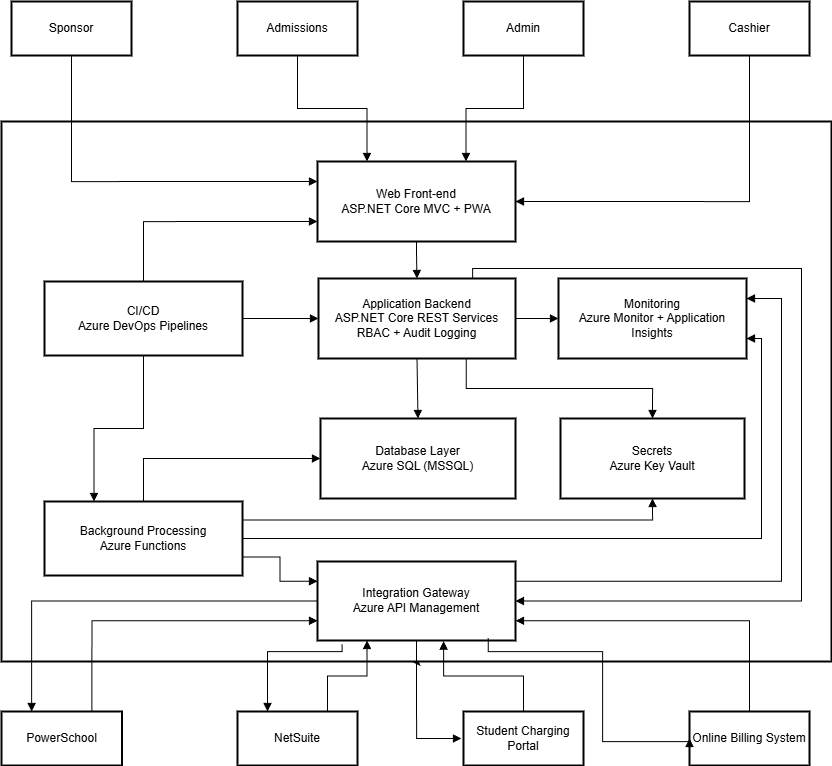
\includegraphics[width=0.88\linewidth]{images/Architecture overview.png}
            \caption{Architecture overview}
            \label{fig:Architecture overview}
        \end{center}
        \end{figure}

        \noindent Figure~\ref{fig:Architecture overview} details the Azure-based pilot architecture, including the role-based web interface, ASP.NET Core application layer, Azure SQL data store, monitoring services, and future API gateway path. The figure is included to show how the deployed pilot can support integration hardening without replacing ISM's existing systems.

        \item \subsubsection{Core Functional Services}
        
        The application offers 5 basic services. \textbf{Sponsor Master Data Management} stores sponsor \textbf{identity}, \textbf{TIN}, \textbf{Address} and \textbf{contact}s, and \textbf{provides controlled updates} and \textbf{approval} when necessary. LoG Rule Authoring can be done on sponsor and student level, allowing for differentiated coverage policies. \textbf{Coverage Evaluation} uses LoG rules to determine the covered/\textbf{bill-to} results for line items to be charged, including a quick preview path for frequently charged items. \textbf{Decision Auditing} captures all evaluation decision information including inputs, rule version, decision reason, user context and time/date of evaluation decision. Identifier Synchronization provides a consistent identifier for students and sponsors between \textbf{PowerSchool}, \textbf{SCP}, \textbf{NetSuite} and \textbf{OBS} to avoid mismatching coverage behavior.
     
        \item \subsubsection{Data Model and Persistence}
        
        Sponsor master records, contact records, LoG rule definitions, rule versions, effective date ranges, student-specific overrides, LoG instances per student per school year, and coverage results that are used by downstream billing are all stored in Azure SQL. audit log tables record each decision and important user action along with before/after values of changes. Sync status, last successful sync time, number of retries, and error information are stored in integration tracking tables to aid in operational visibility.
        
        %Sponsor Management ERD
        \begin{figure}[H]
            \centering
            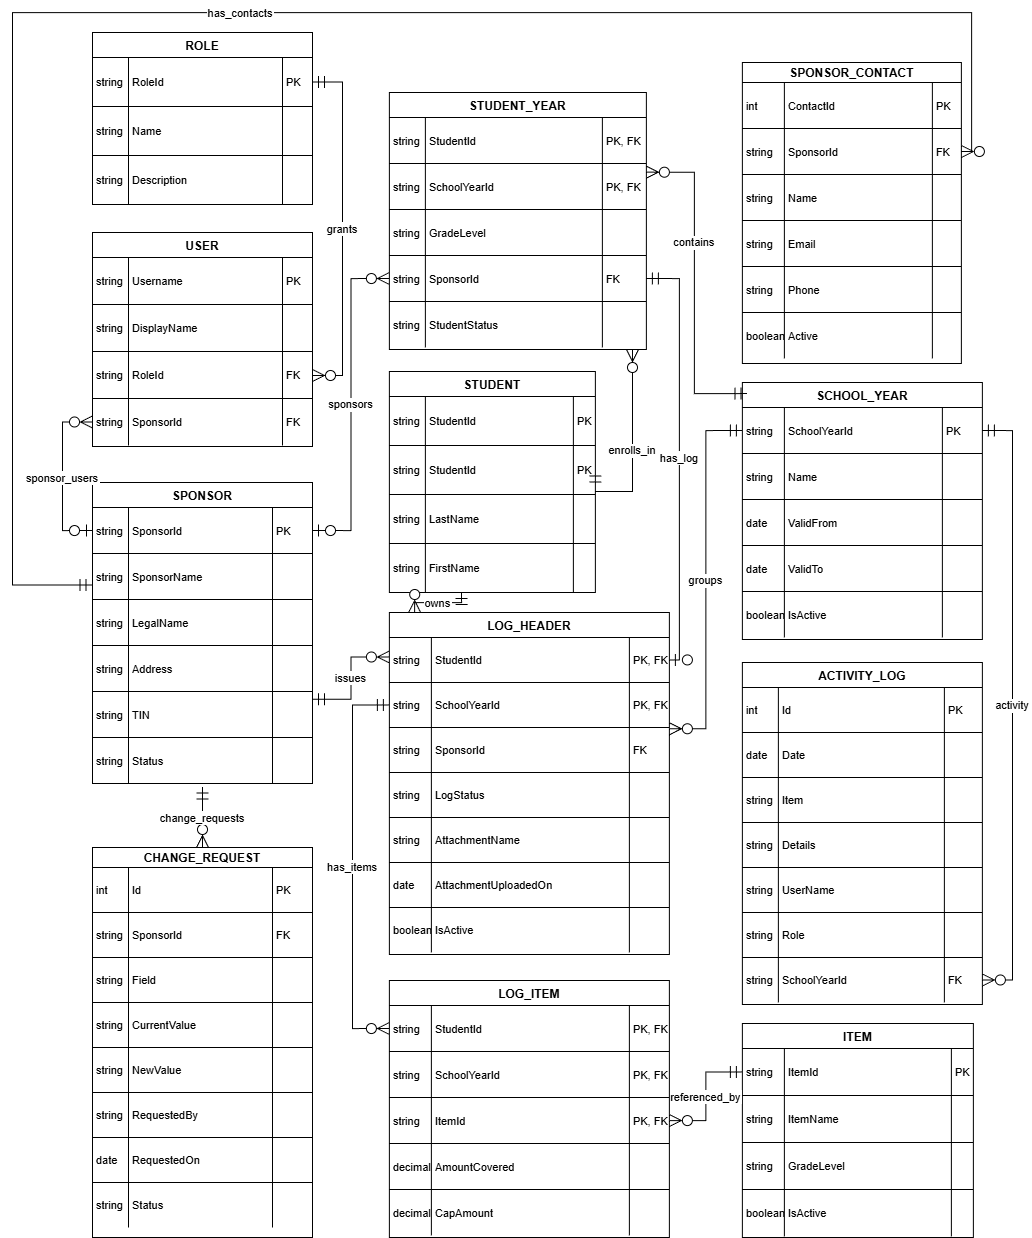
\includegraphics[height=0.72\textheight,keepaspectratio]{images/Proposal ERD.png}
            \caption{Sponsor Management ERD}
            \label{fig:Sponsor Management ERD}
        \end{figure}

        \noindent Figure~\ref{fig:Sponsor Management ERD} details the logical data model used by the pilot, including sponsors, contacts, users, roles, students, school years, LoG records, LoG items, charge requests, items, and activity logs. The figure is included to show how sponsor identity, coverage rules, and audit records are connected in the system database.
        
        \item \subsubsection{Coverage Computation and \textbf{Bill-To} Determination}
        
        System determines if a student is covered by the sponsor at charge line-level, based on deterministic rules based on the sponsor's LoG, and/or any student specific overrides. The result of each evaluation is a coverage classification and an authoritative Bill-To designation along with sponsor-parent allocation amounts and percentages and an auditable explanation of the reason code and rule version used for the evaluation. Student Identifier, Sponsor Identifier, School Year, Charge Item Code, Charge Category, Charge Amount, Charge Date, LoG effective date range, coverage caps or limits, exclusions, required documentation flags and student level overrides are inputs to the evaluation. The evaluation takes care of rule priority so that no two rules can have the same effect and result in an ambiguous or conflicting outcome.
        
        The coverage outcomes are defined as: (a) \textbf{Covered} – the sponsor is responsible for 100\% of the amount subject to the coverage caps and effective dates; (b) \textbf{Split} – the parent and sponsor are responsible for the amount subject to the coverage caps and effective dates following the rules defined herein; and (c) \textbf{Not Covered} – the parent is responsible for the amount subject to the coverage caps and effective dates.
        
        The explicit formulas are used to compute the allocation. In case of a cap based split, the system proceeds to calculate the following: SponsorCoveredAmount = min(ChargeAmount, RemainingCap) and ParentAmount = ChargeAmount - SponsorCoveredAmount. Percent allocations are calculated by dividing the amount covered by the Sponsor by the ChargeAmount (SponsorPercent) and the amount covered by the Parent by the ChargeAmount (ParentPercent). The monetary and percentage allocation to support downstream billing and reconciliation is recorded in the system.
        
        Bill-To is based on the calculated allocation. When SponsorPercent = 1.00, then Bill-To = Sponsor. SponsorPercent 0.00, Bill-To is Parent. If SponsorPercent is in the range 0.00 – 1.00, then Bill-To is Split and the explicit sponsor and parent allocations are propagated to downstream systems. For each decision a reason code and a rule version is persisted, so as to be traceable and auditable.
        
        \item \subsubsection{Integration Design}
        
        This is a sequence diagram of the real time interaction between systems in entering a charge. Student Charging Portal makes a Coverage API request to make a preview decision. The Coverage API queries the Sponsor Master for LoG and rule data, attempts to make a decision with allocations and audit data, and the portal pushes allocations to NetSuite and updates the Online Billing System (OBS) for statements to be displayed.
        
        %Integration Interaction Flow
        \begin{figure}[H]
            \centering
            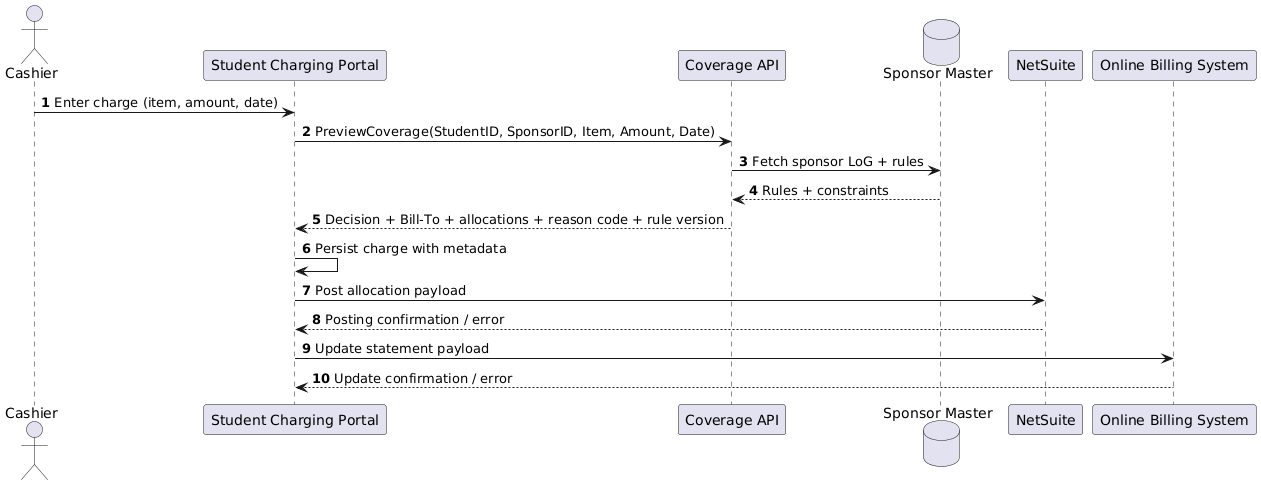
\includegraphics[width=0.98\linewidth]{images/integration flow.png}
            \caption{Integration Interaction Flow}
            \label{fig:Integration Interaction Flow}
        \end{figure}

        \noindent Figure~\ref{fig:Integration Interaction Flow} details the intended interaction between the Student Charging Portal, the coverage API, the Sponsor Master, NetSuite, and the Online Billing System. The figure is included to show how a charge entry can be evaluated once and then passed downstream with decision metadata and sponsor-parent allocation details.

        \item \subsubsection{Integration as the Core Implementation Component}
        
        The integration, as a core implementation component, is a structured approach that integrates materials and resources.
        
        An important aspect of the deployed pilot web application was the design of the integration that linked sponsor data, the coverage rules for LoG, the data about students, the decisions on charges, as well as outputs to the billing system across the existing ISM system landscape. The project was not designed to supplant or replace PowerSchool, NetSuite, the Student Charging Portal or the Online Billing System. It did, however, add a centralized Sponsor Master and coverage decision layer which could act as a common reference point for these systems.
        
        The integration part was crucial because the consistent identifiers and consistent interpretation of LoG provisions are necessary to sponsorship billing. The absence of a common integration layer means that names of sponsors, student records, charge categories, limits of expenditure (LoG) and assignments to a Bill-To can vary in meaning from one department to another and from one application to another. This problem was resolved by the deployed pilot who collected all the sponsor records, LoG records, coverage rules, audit records and downstream billing references into one application model.
        
        The pilot implementation confirmed the validity of the idea of integration via REST API endpoints, sponsor and LoG data structure, coverage preview response, audit decision records and synchronization-ready data structures. While integration with live production with PowerSchool, NetSuite and Online Billing System was not completely finished with the pilot scope, the application that was deployed provided the technical groundwork for future system to system exchange. This comprised of canonical sponsor identifiers, student references, LoG status fields, coverage-result structures, audit metadata and integration status endpoints.
        
        This integration-focused design allows for the project goal of delivering consistent, explainable and auditable coverage decisions with no requirement to replace ISM's enterprise systems. It also offers a pragmatic way to go forward with future production activities where API configuration, scheduled synchronization, error handling and reconciliation reports can be done and can be compared with live or staging institutional data. The supporting API and integration-readiness evidence is placed in \hyperref[app:integration-evidence]{Appendix A.6}.
     
        \setlength{\LTleft}{0pt}
        \setlength{\LTright}{\fill}
        \begin{longtable}{>{\raggedright\arraybackslash}p{0.22\linewidth}
                    >{\raggedright\arraybackslash}p{0.30\linewidth}
                    >{\raggedright\arraybackslash}p{0.40\linewidth}}
        \caption{Critical integration components of the deployed pilot web application}\label{table:critical-integration-components}\\
        \toprule
        \textbf{Integration component} & \textbf{Purpose} & \textbf{Pilot implementation evidence} \\
        \midrule
        \endfirsthead
        \caption[]{Critical integration components of the deployed pilot web application (continued)}\\
        \toprule
        \textbf{Integration component} & \textbf{Purpose} & \textbf{Pilot implementation evidence} \\
        \midrule
        \endhead
        \midrule
        \multicolumn{3}{r}{\textit{Continued on next page}}\\
        \endfoot
        \bottomrule
        \endlastfoot
        Sponsor Master & Provides the canonical sponsor reference used by staff and sponsor-facing workflows. & Sponsor CRUD, duplicate prevention, sponsor profile management, sponsor contacts, and SponsorID-based records. \\
                    LoG Management & Maintains sponsor coverage documents, effective dates, statuses, and coverage-related rules. & LoG list, create LoG workflow, activation status, coverage fields, and sponsor-facing LoG views. \\
                    Coverage Evaluation & Produces consistent coverage outcomes for charge-related decisions. & Coverage preview API, reason codes, \textbf{Bill-To} outcome, sponsor and parent allocation fields, and audit record generation. \\
                    Audit Trail & Records decision and activity evidence for traceability and review. & Audit decision endpoint, activity logs, timestamps, rule references, and user action records. \\
                    External System Readiness & Prepares the application for future PowerSchool, NetSuite, Student Charging Portal, and Online Billing System synchronization. & REST API structure, integration status endpoint, mapped identifiers, Azure deployment, and synchronization-ready data model. \\
        \end{longtable}
        
        Table~\ref{table:critical-integration-components} shows why integration was treated as a core implementation component. The table connects each integration function to specific pilot evidence, showing that the web application was not merely a sponsor portal but a foundation for consistent system-to-system sponsorship billing governance.
        \pagebreak
        
        \item \subsubsection{Per-Application Activity Diagram}
        
        \textbf{PowerSchool Activity (Student Record and Sponsor Tagging).} This activity diagram outlines the student identity and sponsor linkage for PowerSchool. Staff create or update student records, add a SponsorID or sponsorship indicator, validate sponsor association and sync the student-sponsor relationship to the Sponsor Master. If the student is not connected to a sponsor, the student is parent responsible by default.
                 
        %PS Activity
        \begin{figure}[H]
        \begin{center}
            \vspace{2ex}
            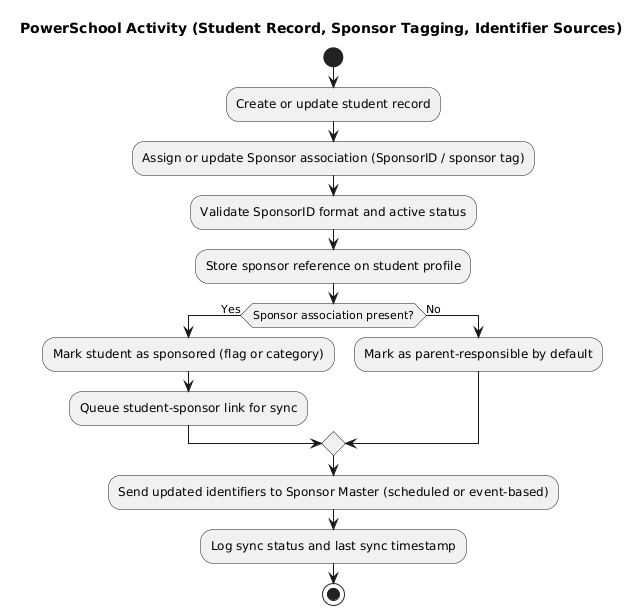
\includegraphics[width=350pt]{images/PS Activity.png}
            \caption{PowerSchool Activity}
            \label{fig:PowerSchool Activity}
        \end{center}
        \end{figure}

        \noindent Figure~\ref{fig:PowerSchool Activity} details the PowerSchool-related activity flow, where student identity and sponsor tagging provide the source linkage for sponsor-student association. The figure is included to show why consistent sponsor identifiers are needed before LoG coverage can be evaluated reliably.

        \textbf{Student Charging Portal Activity (Charge Entry and Coverage Preview).} This activity diagram illustrates the decisions that can be made at the point of charge entry which are supported by the Student Charging Portal. The user enters the charge information, asks for a coverage preview and obtains a coverage determination including allocations for sponsors and parents. The user agrees to this decision and the charge is posted with decision meta data to downstream systems. Otherwise, the user tweaks the inputs and preview runs again.
        
        %Student Charging Portal Activity
        \begin{figure}[H]
        \begin{center}
            \vspace{2ex}
            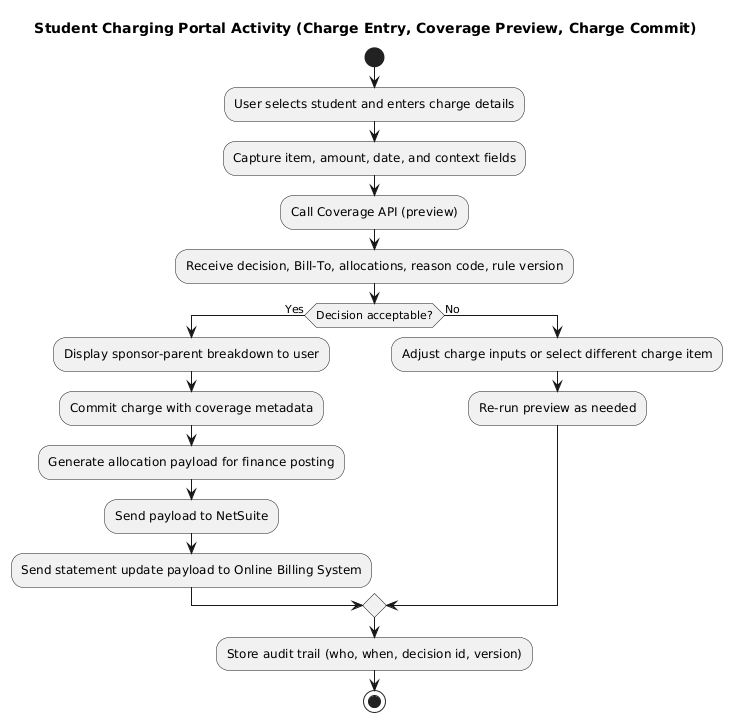
\includegraphics[width=350pt]{images/SCP Activity.png}
            \caption{Student Charging Portal Activity}
            \label{fig:Student Charging Portal Activity}
        \end{center}
        \end{figure}

        \noindent Figure~\ref{fig:Student Charging Portal Activity} details the charge-entry workflow in which the Student Charging Portal requests a coverage preview, receives a Bill-To decision, and commits the charge with decision metadata. The figure is included to show how manual LoG interpretation is replaced by repeatable rule-based validation at the point of charge entry.

        \textbf{NetSuite Activity (Allocation Posting and Receivables).} This activity diagram illustrates how NetSuite gets the allocation results and posts them as Receivables. NetSuite validates the payload, sets AR transaction lines for sponsor and parent portions, adds the decision metadata for Auditability and returns confirmation. Bad payloads are refused with error information and they are logged for debugging purposes.
        
        %NetSuite Activity
        \begin{figure}[H]
        \begin{center}
            \vspace{2ex}
            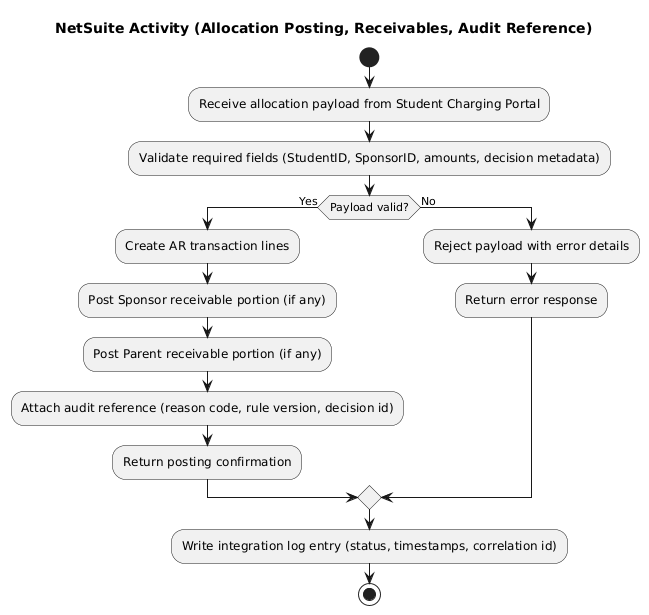
\includegraphics[width=350pt]{images/NetSuite Activity.png}
            \caption{NetSuite Activity}
            \label{fig:NetSuite Activity}
        \end{center}
        \end{figure}

        \noindent Figure~\ref{fig:NetSuite Activity} details how sponsor-parent allocation results would be validated and posted to NetSuite as receivable lines with audit references. The figure is included to show how the finance system can receive structured billing outcomes instead of manually interpreted charge assignments.

        \textbf{Online Billing System Activity (Statement Presentation).} This activity diagram depicts the Online Billing System's presentation of the billing outcome to the end users. It takes statement updates, validates the update, adds charge lines and sponsor-parent allocations and publishes an updated statement. It even includes the revision history and integration correlation identifiers for traceability.
       
        %Online Billing System Activity
        \begin{figure}[H]
        \begin{center}
            \vspace{2ex}
            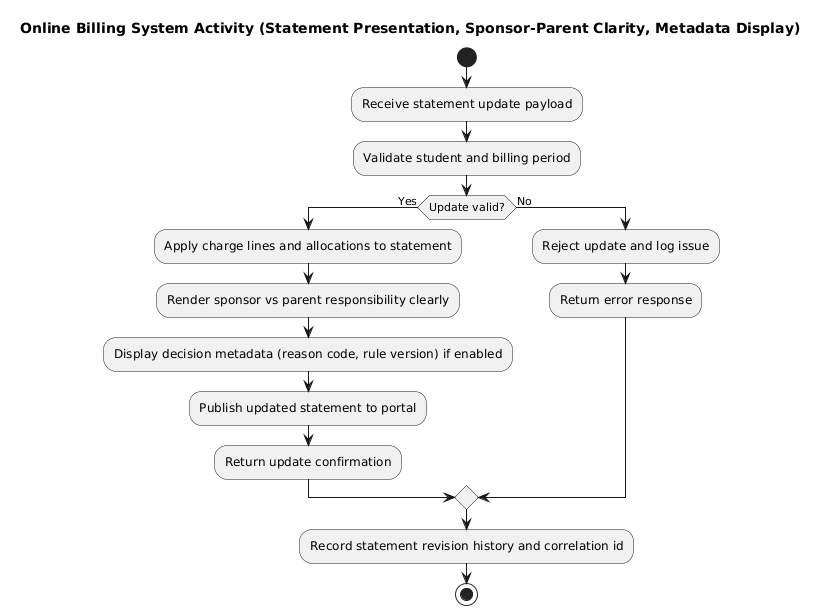
\includegraphics[width=350pt]{images/Online Billing System Activity.png}
            \caption{Online Billing System Activity}
            \label{fig:Online Billing System Activity}
        \end{center}
        \end{figure}

        \noindent Figure~\ref{fig:Online Billing System Activity} details how the Online Billing System would receive statement updates, apply charge lines and sponsor-parent allocations, publish updated statements, and retain revision history. The figure is included to show how the final billing view can reflect the same coverage decision produced during charge entry.

        \item \subsubsection{Cross-System Data Mapping and ERD Integration View}
        
        The integration view defines all the canonical student, sponsor, charge and allocation identifiers that are used to connect student, sponsor, charge and allocation records across systems. For those vendor schemas that have not been made available, or are proprietary, the manuscript supplies a logical view of the ERD integration showing emphasis on join keys, mapping fields and the direction of the synchronization.
       
        \setlength{\LTleft}{0pt}
        \setlength{\LTright}{\fill}
        Table~\ref{table:role-functions} lists the logical entities and key identifiers used to align sponsor, student, charge, and allocation data across the connected systems.
        
        \begin{longtable}{>{\raggedright\arraybackslash}p{0.18\linewidth}
                    >{\raggedright\arraybackslash}p{0.17\linewidth}
                    >{\raggedright\arraybackslash}p{0.21\linewidth}
                    >{\raggedright\arraybackslash}p{0.19\linewidth}
                    >{\raggedright\arraybackslash}p{0.17\linewidth}}
        \caption{Logical cross-system entity mapping and key identifiers}\label{table:role-functions}\\
        \toprule
        \textbf{Entity} & \textbf{PowerSchool (SIS)} & \textbf{Student Charging Portal} & \textbf{NetSuite (ERP)} & \textbf{Online Billing System} \\
        \midrule
        \endfirsthead
        \caption[]{Logical cross-system entity mapping and key identifiers (continued)}\\
        \toprule
        \textbf{Entity} & \textbf{PowerSchool (SIS)} & \textbf{Student Charging Portal} & \textbf{NetSuite (ERP)} & \textbf{Online Billing System} \\
        \midrule
        \endhead
        \midrule
        \multicolumn{5}{r}{\textit{Continued on next page}}\\
        \endfoot
        \bottomrule
        \endlastfoot
        \textbf{Student} & StudentID (authoritative) & StudentID (reference) & Customer/Student key (mapped) & Student account key (mapped) \\
                    \textbf{Sponsor} & Sponsor reference (if present) & SponsorID (reference) & CustomerID (mapped) & Sponsor account key (mapped) \\
                    \textbf{LoG} & Document reference (optional) & LoG record (reference) & Not stored as LoG (reference via audit id) & Displayed metadata (reference) \\
                    \textbf{Charge Line} & Optional fee definition & ChargeLineID (authoritative at entry) & Transaction/Invoice line key (mapped) & Statement line key (mapped) \\
                    \textbf{Allocation} & Not computed & Allocation fields (authoritative) & Accounting split fields (mapped) & Displayed split fields (mapped) \\
        \end{longtable}
                
        \item \subsubsection{Workflow Alignment}
        
        Sponsor onboarding starts with staff creation or submission of sponsor details and necessary documentation, and approval if applicable. Sponsor Identifiers are added and available in PowerSchool and downstream systems upon approval. Sponsor OrgName tagging in PowerSchool is the basis for student sponsor assignment, which is synced to NetSuite, OBS and SCP. LoG rules and/or student-level LoG coverage is defined and stored in the application and a decision to cover the charge line item is determined and recorded and synched to use for billing.

        %Context Diagram
        \begin{figure}[H]
        \begin{center}
            \vspace{2ex}
            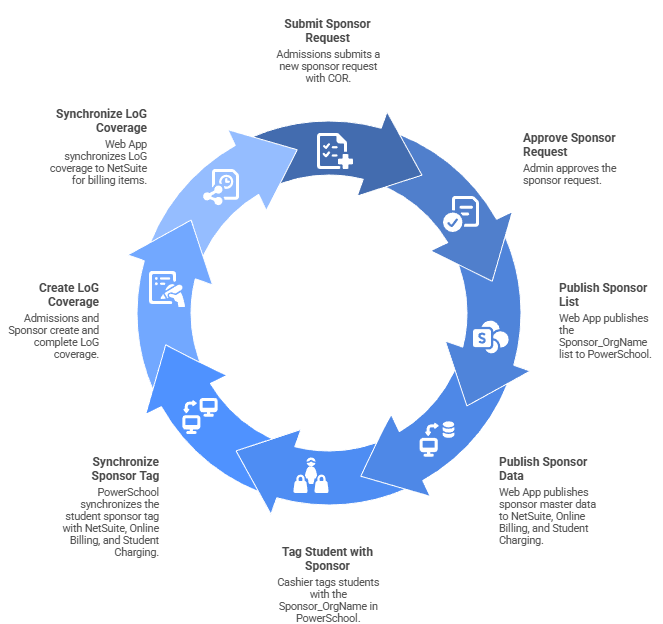
\includegraphics[width=400pt]{images/Context Diagram.png}
            \caption{Context Diagram}
            \label{fig:Context Diagram}
        \end{center}
        \end{figure}

        \noindent Figure~\ref{fig:Context Diagram} details the end-to-end context for sponsor requests, approvals, sponsor data publication, student tagging, LoG coverage synchronization, and billing outputs. The figure is included to show how the pilot sits between sponsor users, staff users, and the existing ISM system landscape.
    \end{itemize}
    \pagebreak
    
    \subsection{Implementation}
    
    The implementation involved three parallel threads:
    
    \begin{enumerate}
        \item Sponsor Master CRUD with contacts and addresses, name uniqueness checks against TIN and cross system-id.
        \item Create and Edit actions per student, with per student rules, caps and effective dates, status changes and notes.
        \item Functions in Coverage API that determine if a mock charge line qualifies for coverage and return decision along with reason codes and audit entries.
    \end{enumerate}
    
    The deployment was done with Azure DevOps pipelines and the deployment was Build to Test to Deploy to Dev to Manual Approval to Deploy to Pilot. De-identified records were used in the pilot data. The success measures were a decrease in manual checks, a decrease in reversals, and consistent Bill-To assignment at invoice creation.
 
    \subsection{User Interface Implementation}
    
    The User Interface of the \textbf{deployed pilot web application} was made to match with the current running Azure pilot application. It features a responsive role-based layout, a shared sign-in page, sidebar navigation that's role-aware, dashboard-specific views, and internal and sponsor-facing modules. The interface is responsive and PWA; but, it was not implemented as a full PWA as Installable offline behavior, service-worker caching, and a production web app manifest were not enabled in the pilot.
    
    The screenshots of the interface in this section have been inserted in the respective topics. This helps avoid the impression of a collection of visuals “displays” and enables the individual figure to validate the discussion in the body of the manuscript.
 
    \setlength{\LTleft}{0pt}
    \setlength{\LTright}{\fill}
    \begin{longtable}{>{\raggedright\arraybackslash}p{0.34\linewidth}
            >{\raggedright\arraybackslash}p{0.58\linewidth}}
    \caption{Interface topics and figure placement}\label{table:interface-visual-placement}\\
    \toprule
    \textbf{Interface topic} & \textbf{Figures placed in the manuscript} \\
    \midrule
    \endfirsthead
    \caption[]{Interface topics and figure placement (continued)}\\
    \toprule
    \textbf{Interface topic} & \textbf{Figures placed in the manuscript} \\
    \midrule
    \endhead
    \midrule
    \multicolumn{2}{r}{\textit{Continued on next page}}\\
    \endfoot
    \bottomrule
    \endlastfoot
    Login and responsive layout & Current ISM Sponsor Management sign-in page. \\
            Dashboard views & Administrator, Admissions, Cashier, and Sponsor dashboards. \\
            Sponsor and contact management & All Sponsors, Create Sponsor, All Contacts, Sponsor Profile, and Sponsor Contacts pages. \\
            Letters of Guarantee and coverage views & Internal LoG list, Create LoG page, sponsor-facing LoG page, and sponsor-facing Students page. \\
            Change requests and sponsor self-service & Sponsor Change Requests and Add New Contact pages. \\
            Reports and monitoring views & Administrator Reports and Sponsor Reports pages. \\
            Administrative settings and data maintenance & School Years, Student Management, Items Management, Role Management, and User Management pages. \\
    \end{longtable}

    Table~\ref{table:interface-visual-placement} shows how each screenshot supports a specific part of the interface discussion and confirms that the visual evidence is placed where the related topic is discussed.

    \setlength{\LTleft}{0pt}
    \setlength{\LTright}{\fill}
    \begin{longtable}{>{\raggedright\arraybackslash}p{0.20\linewidth}
            >{\raggedright\arraybackslash}p{0.72\linewidth}}
    \caption{Implemented role-based navigation in the deployed pilot web application}\label{table:implemented-role-navigation}\\
    \toprule
    \textbf{Role} & \textbf{Implemented navigation and accessible modules} \\
    \midrule
    \endfirsthead
    \caption[]{Implemented role-based navigation in the deployed pilot web application (continued)}\\
    \toprule
    \textbf{Role} & \textbf{Implemented navigation and accessible modules} \\
    \midrule
    \endhead
    \midrule
    \multicolumn{2}{r}{\textit{Continued on next page}}\\
    \endfoot
    \bottomrule
    \endlastfoot
    \textbf{Administrator} & Dashboard; All Sponsors; All Contacts; Letters of Guarantee; Reports; School Years; Students; Items; Roles; Users. Administrator dashboard actions also support sponsor review, LoG review queues, duplicate sponsor review, and sponsor record oversight. \\
            \textbf{Admissions} & Dashboard; Letters of Guarantee; Reports. Admissions workflows support sponsor review, draft LoG preparation, activation request, coverage-alignment checking, and coverage tracking. \\
            \textbf{Cashier} & Dashboard; All Sponsors; All Contacts; Letters of Guarantee; Reports. Cashier reporting supports reconciliation and coverage-decision review for billing verification. \\
            \textbf{Sponsor} & Dashboard; Letters of Guarantee; Students; Change Requests; Contacts; My Profile; Reports. Sponsor users can view their own records, submit profile-change requests, and review assigned LoGs and student coverage details. \\
    \end{longtable}

    Table~\ref{table:implemented-role-navigation} justifies the interface discussion because it reflects the current navigation structure shown in the captured application screens. It also confirms that staff-facing administration functions and sponsor-facing self-service functions are separated by role.
    \clearpage

    \subsubsection{Login and Responsive Layout}
    
    The application will start on the ISM Sponsor Management – Sign In page. The page offers an opportunity for staff users to sign in with an ISM Google account, and also offers username/password access for Sponsor Organization users. This is in support of the bi-authentication model that was tested during pilot validation. In order to provide a document of the actual entry point for the deployed pilot web application, Figure~\ref{fig:login-responsive-layout} is placed directly below this topic. It also highlights the distinction between staff readiness to sign in to Google and access via their sponsor's username and password, allowing for the role-based access model validated during testing.

    \begin{figure}[H]
        \centering
        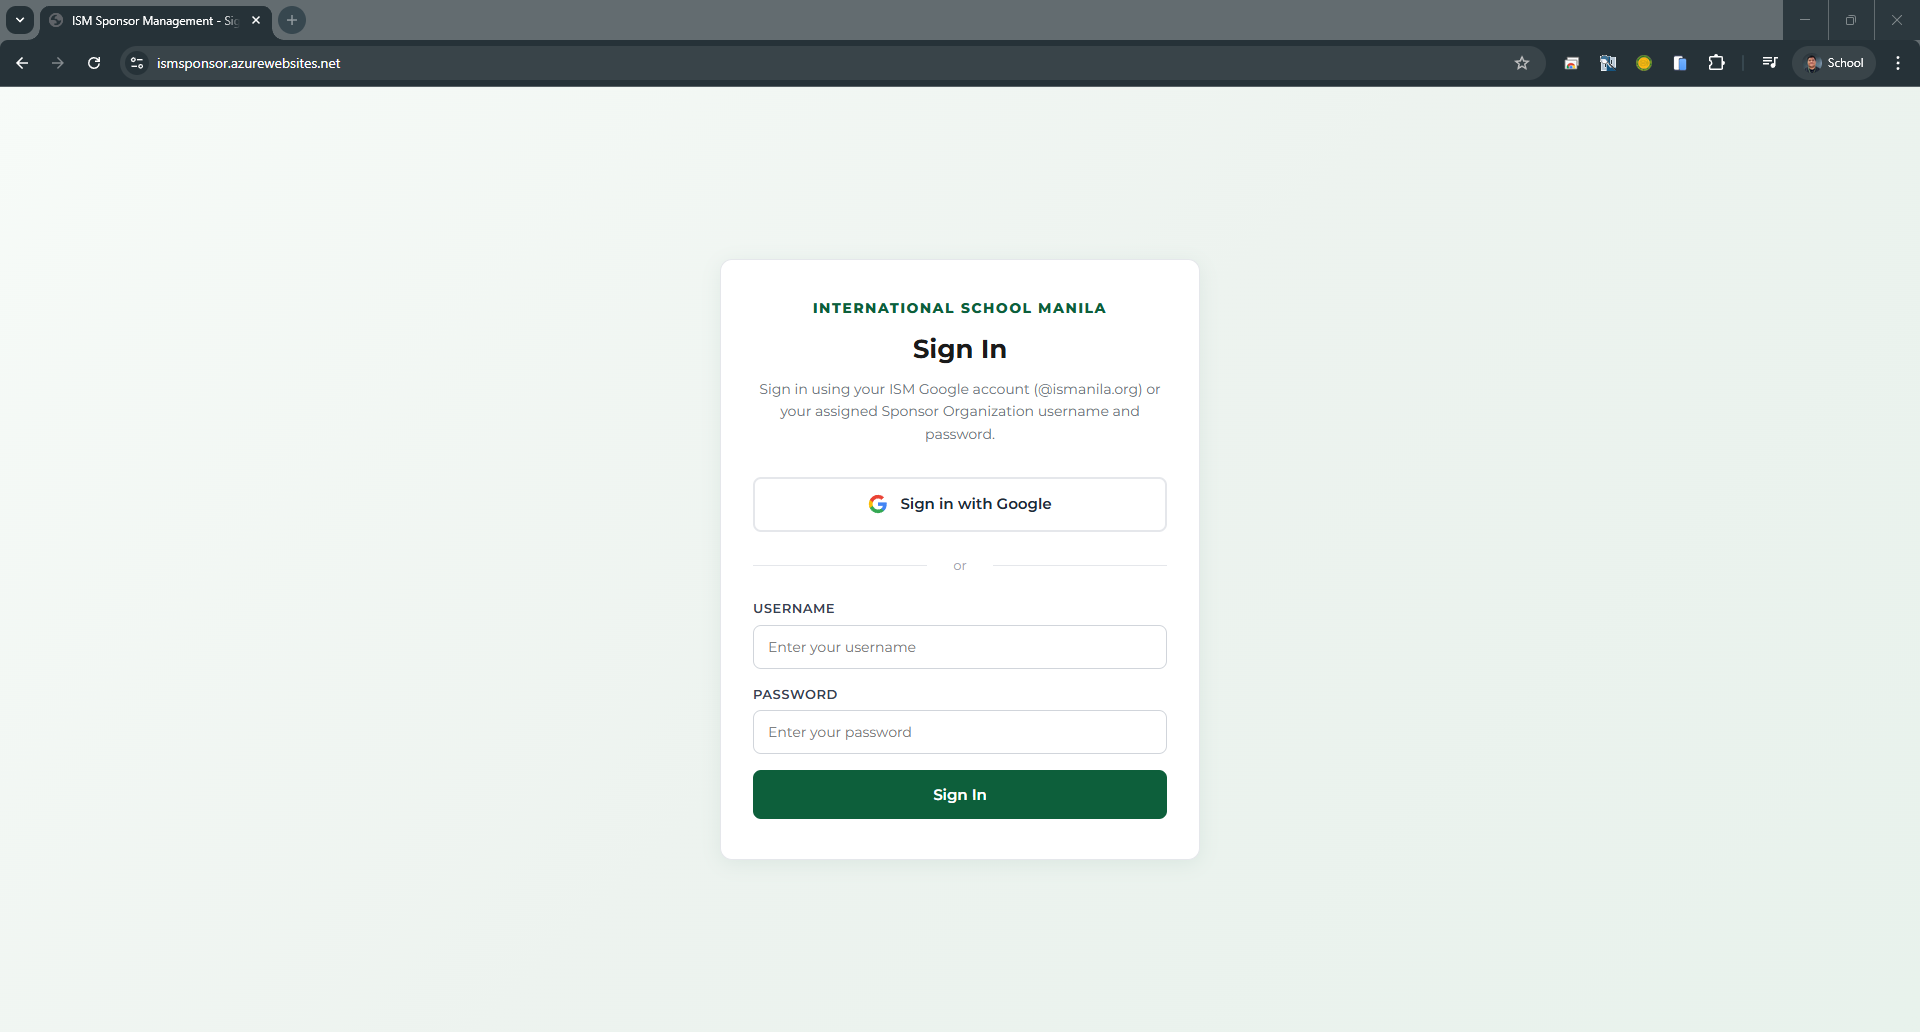
\includegraphics[width=0.90\linewidth]{images/current-interface/admin_login.png}
        \caption{Current ISM Sponsor Management sign-in page}
        \label{fig:current-login-page}
    \end{figure}

    \noindent Figure~\ref{fig:current-login-page} details the shared sign-in page used by internal staff and sponsor users in the deployed pilot. The figure is included to show the entry point for role-based access control, where authenticated users are routed to functions allowed by their assigned role.
    \clearpage

    \subsubsection{Dashboard Views}
    
    The deployed pilot makes available dashboard pages for the role. The indicators on the Administrator dashboard display the status of system-wide indicators of sponsor, LoG, change-request and user-management. Admissions and Cashier dashboards have more restricted views that are relevant to their work. Sponsor users will have their own portal dashboard to focus on their profile, students, Logs and change requests.

    \begin{figure}[H]
        \centering
        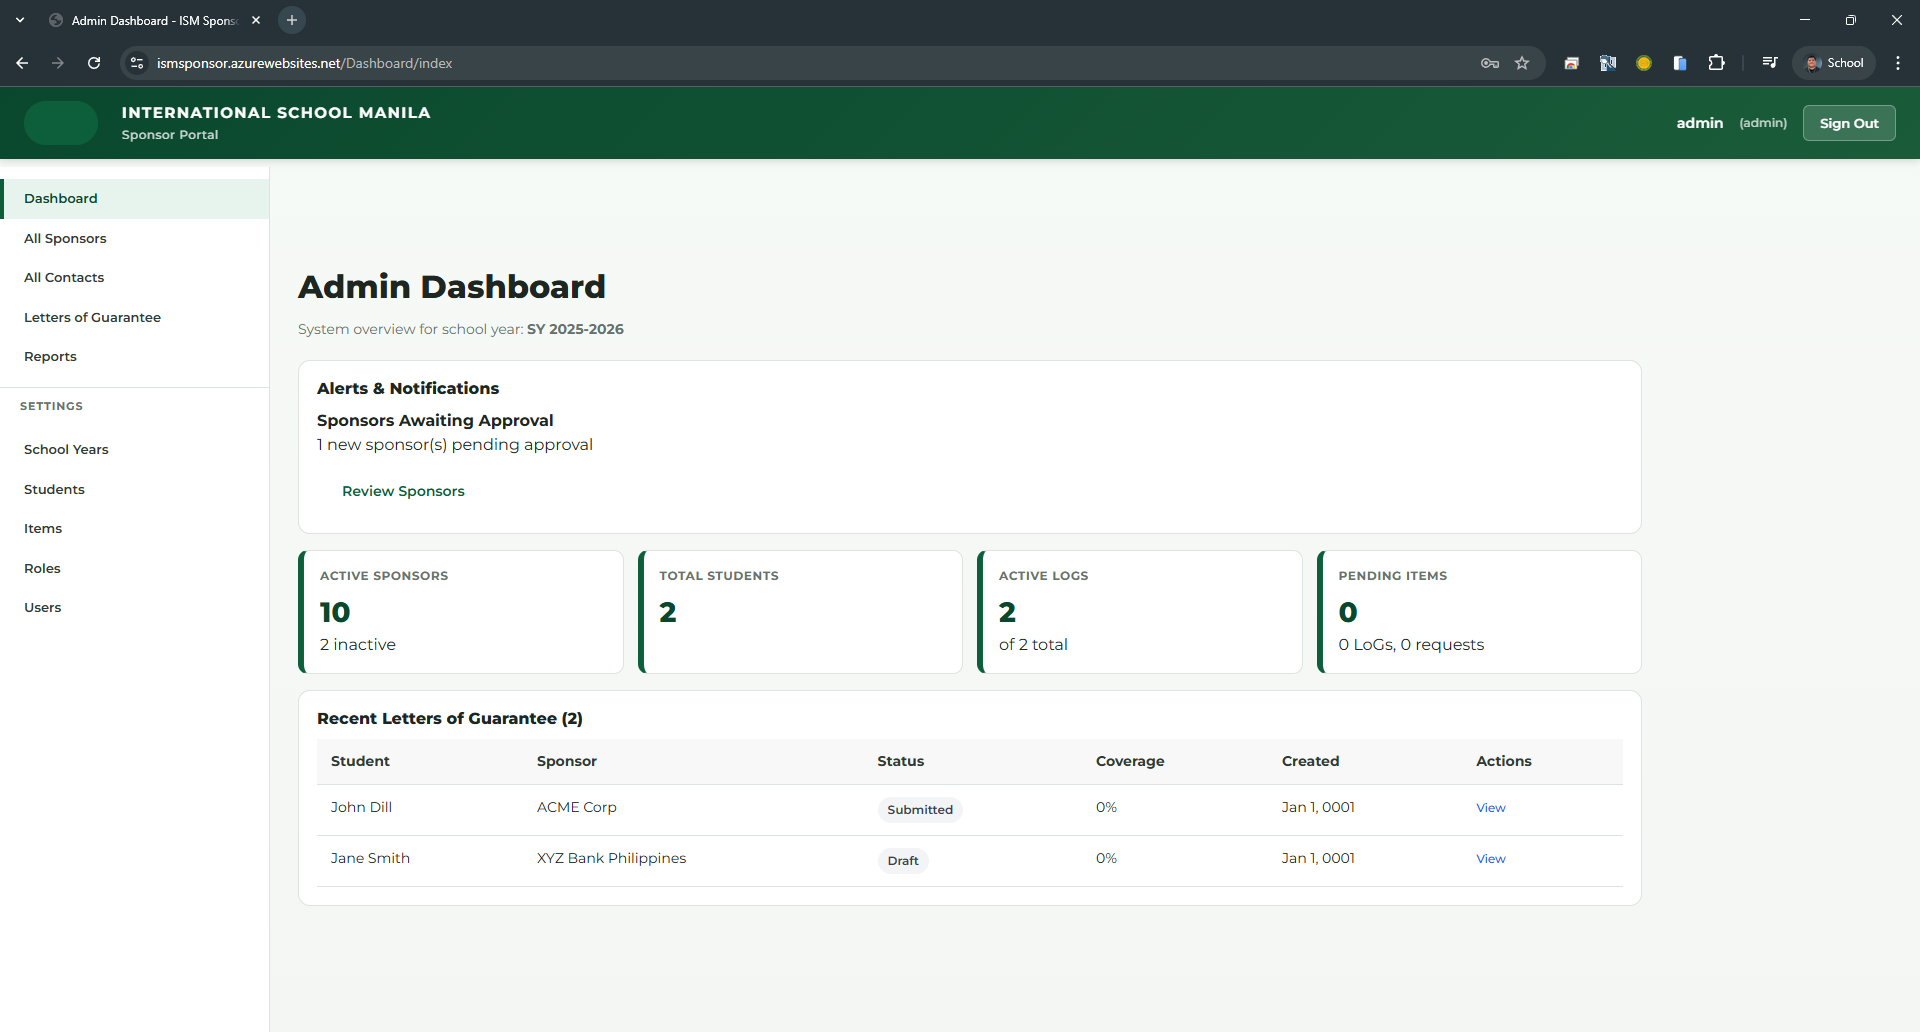
\includegraphics[width=0.90\linewidth]{images/current-interface/admin_dashboard.png}
        \caption{Administrator dashboard in the current deployed pilot web application}
        \label{fig:current-admin-dashboard}
    \end{figure}

    \noindent Figure~\ref{fig:current-admin-dashboard} details the Administrator dashboard, including summary counts, recent activity, and governance-oriented shortcuts for sponsor and LoG oversight. The figure is included to show how administrative users monitor the pilot and control records that affect sponsor billing decisions.

    \begin{figure}[H]
        \centering
        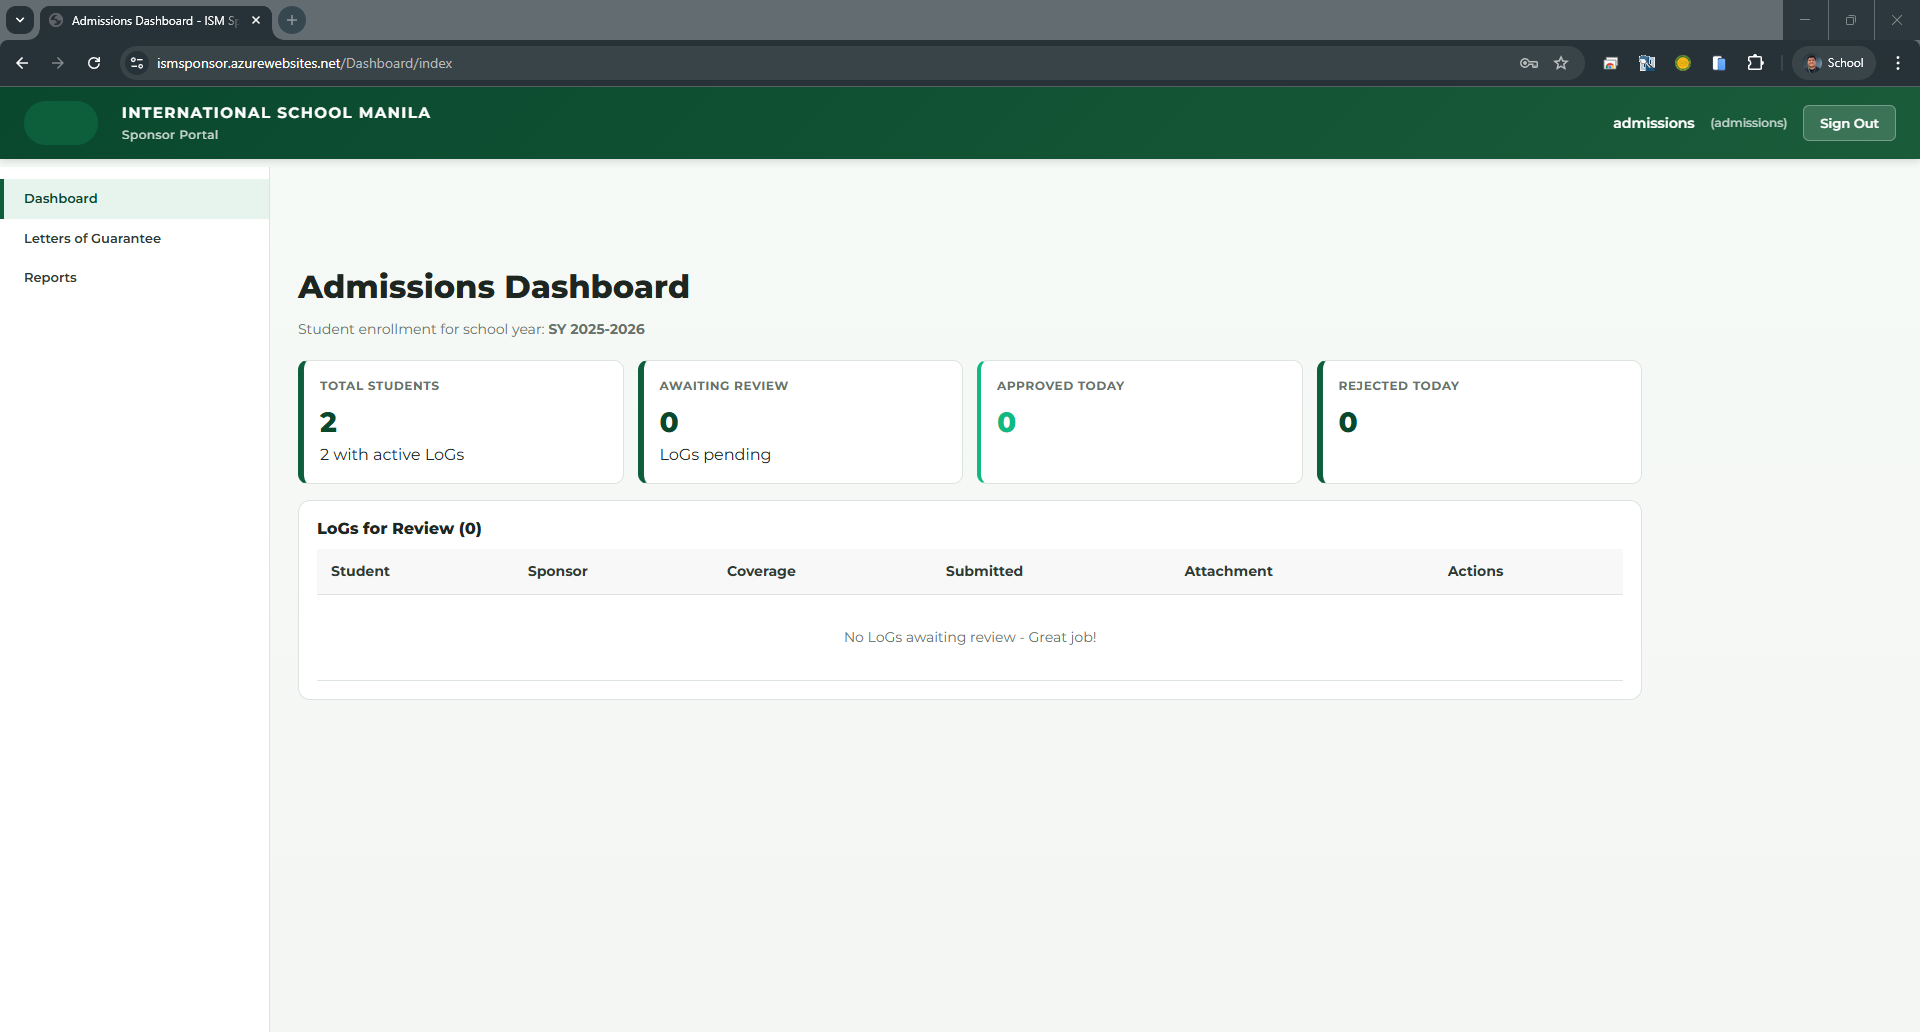
\includegraphics[width=0.90\linewidth]{images/current-interface/admissions_dashboard.png}
        \caption{Admissions dashboard in the current deployed pilot web application}
        \label{fig:current-admissions-dashboard}
    \end{figure}

    \noindent Figure~\ref{fig:current-admissions-dashboard} details the Admissions dashboard, which supports LoG preparation, sponsor review, and pending workflow monitoring. The figure is included to show how admissions-related users can prepare structured coverage information before administrative activation.
    \clearpage
    
    \begin{figure}[H]
        \centering
        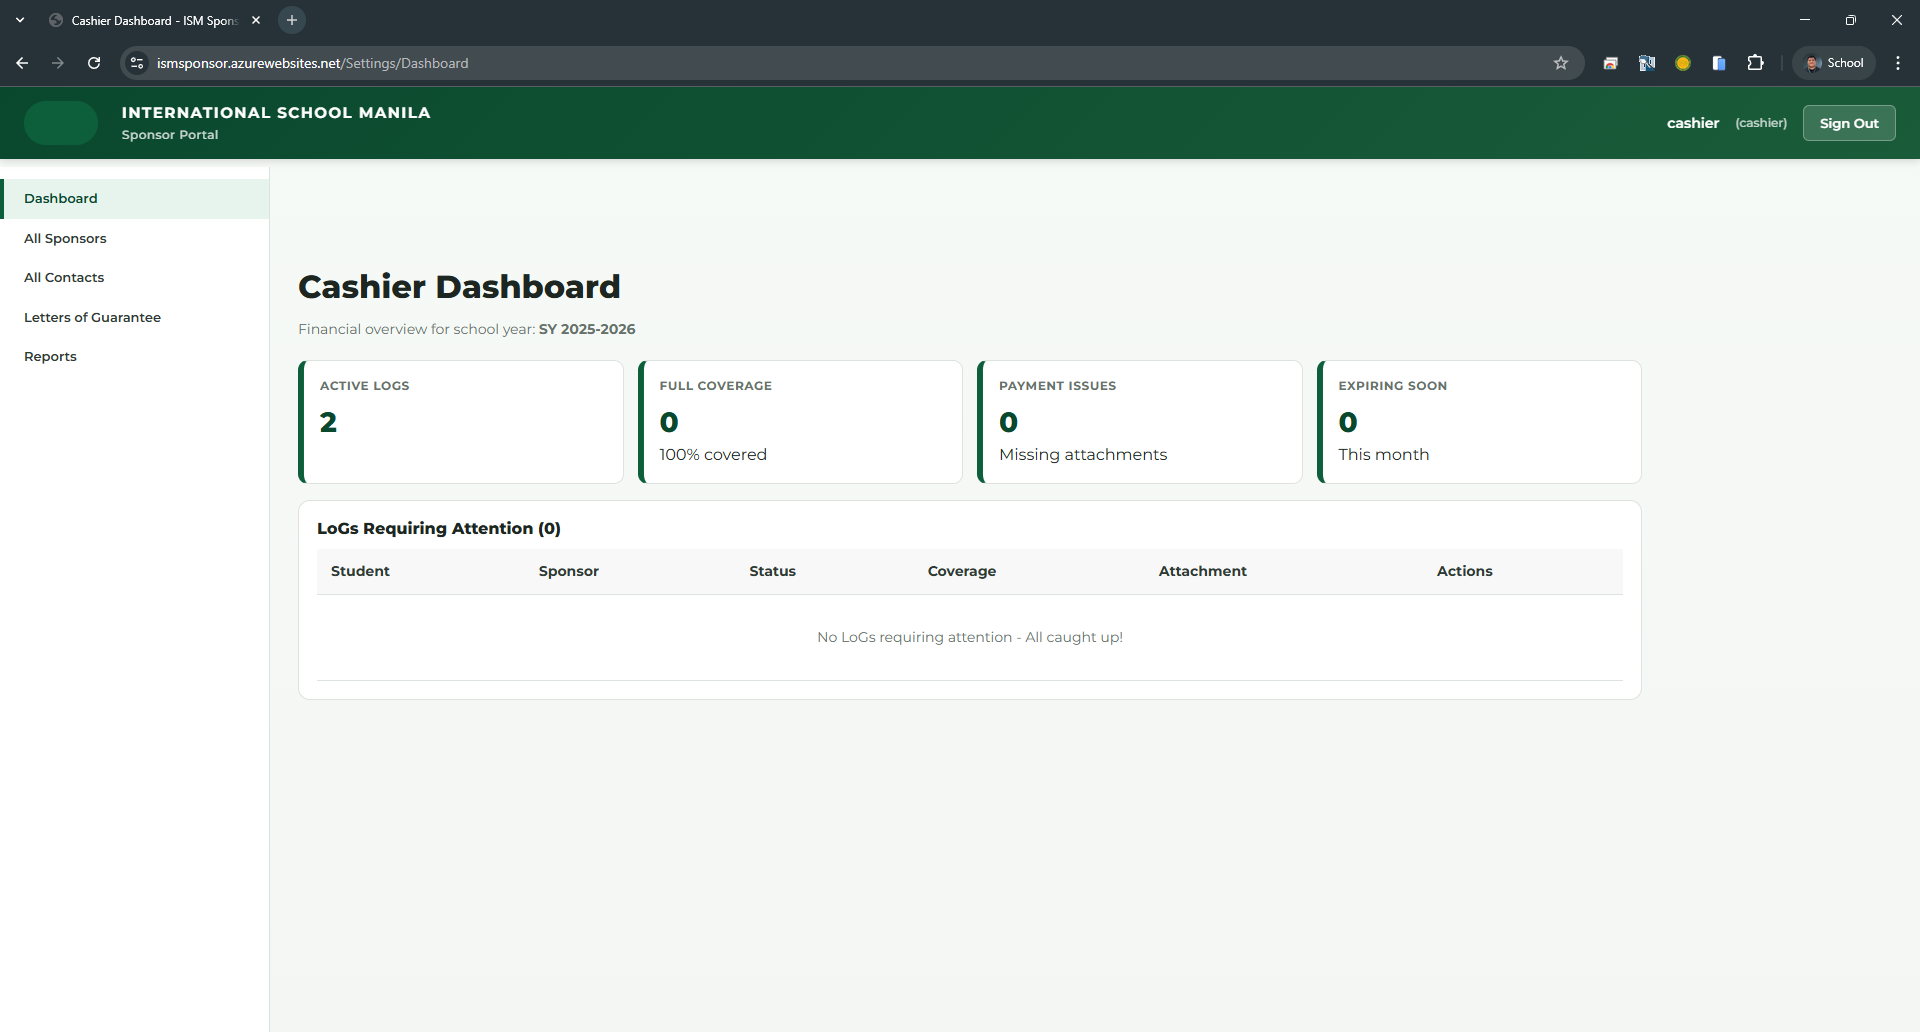
\includegraphics[width=0.90\linewidth]{images/current-interface/cashier_dashboard.png}
        \caption{Cashier dashboard in the current deployed pilot web application}
        \label{fig:current-cashier-dashboard}
    \end{figure}

    \noindent Figure~\ref{fig:current-cashier-dashboard} details the Cashier dashboard, which supports billing review, sponsor lookup, and reconciliation-related LoG monitoring. The figure is included to show how cashier users can verify sponsor and coverage information before or after charge processing.

    \begin{figure}[H]
        \centering
        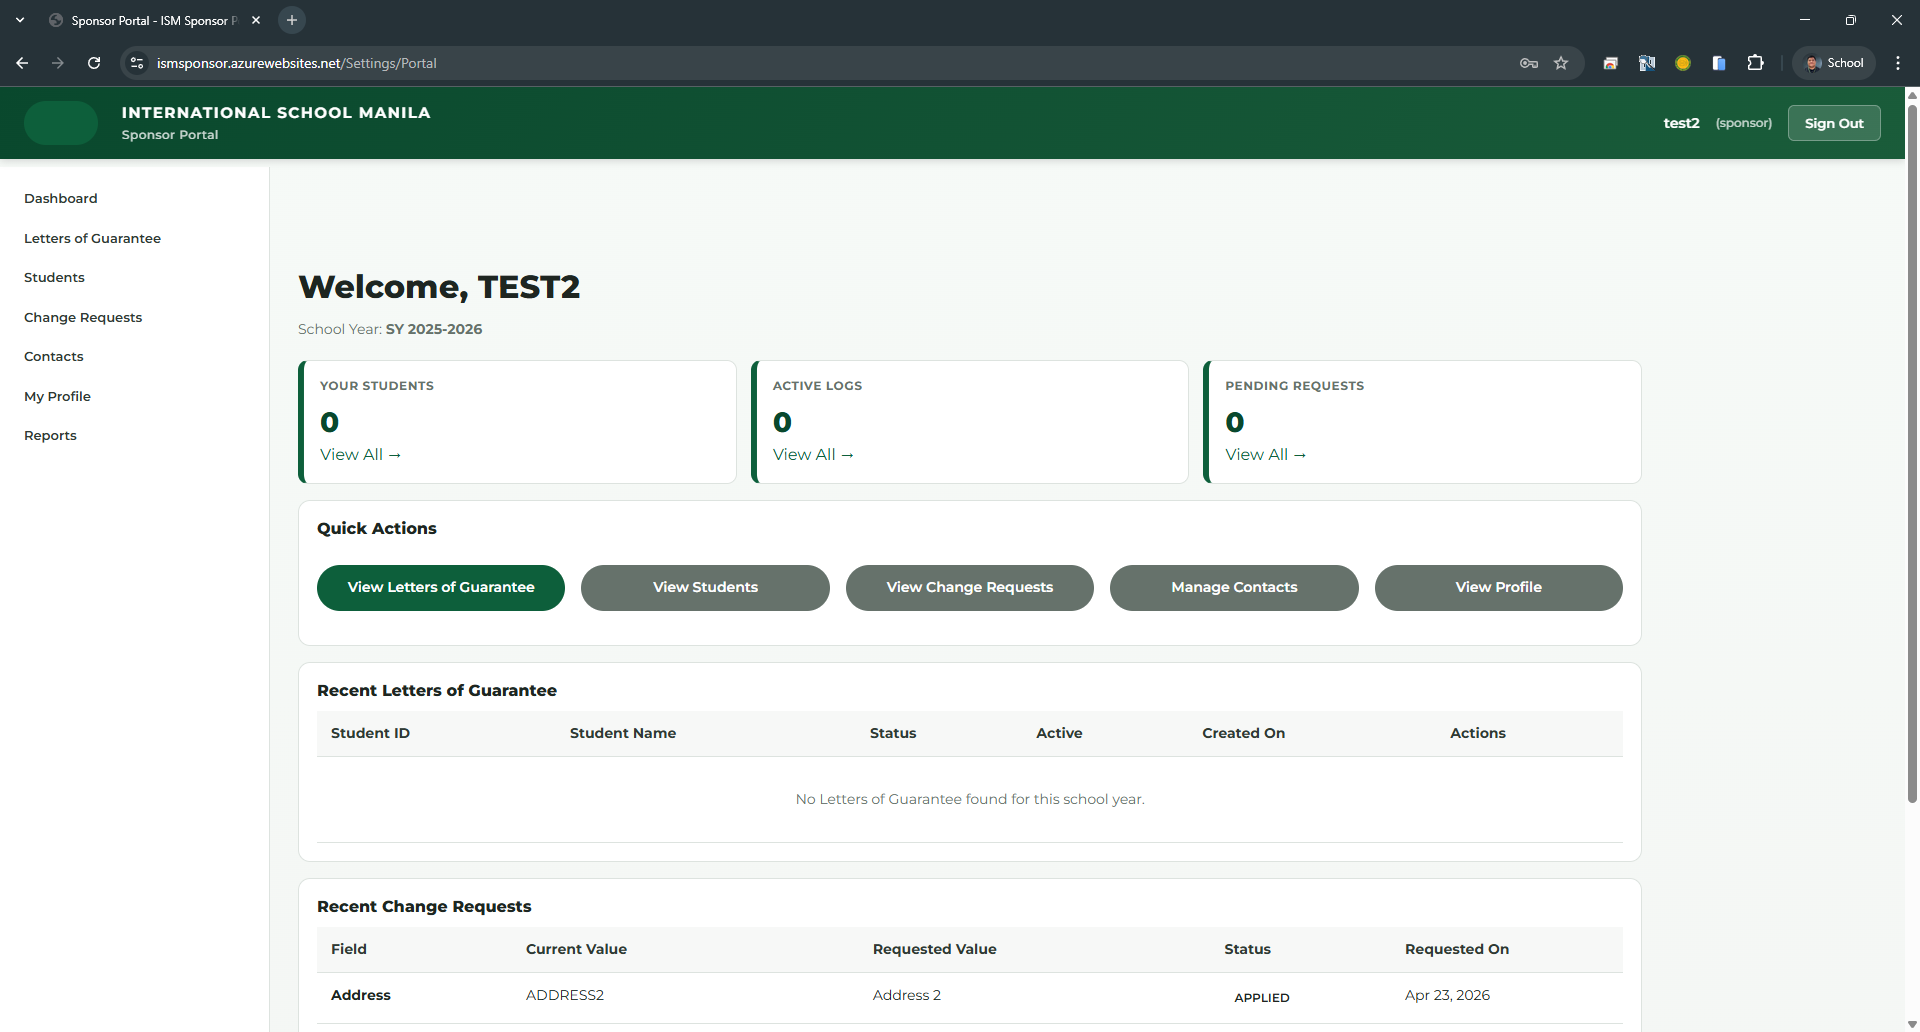
\includegraphics[width=0.90\linewidth]{images/current-interface/sponsor_dashboard.png}
        \caption{Sponsor dashboard in the current deployed pilot web application}
        \label{fig:current-sponsor-dashboard}
    \end{figure}

    \noindent Figure~\ref{fig:current-sponsor-dashboard} details the Sponsor dashboard, which limits visible information to the sponsor's own profile, students, LoGs, requests, and reports. The figure is included to show how the portal supports sponsor self-service while maintaining data boundaries.
    \clearpage

    \subsubsection{Sponsor and Contact Management}
    
    The management of the Sponsor is done via the All Sponsors module for authorized internal users, and via My Profile for Sponsor users. Administrator User roles can view, search and create sponsor records, whereas Sponsor User roles can only see their own profile and associated contact information.
    
    \begin{figure}[H]
        \centering
        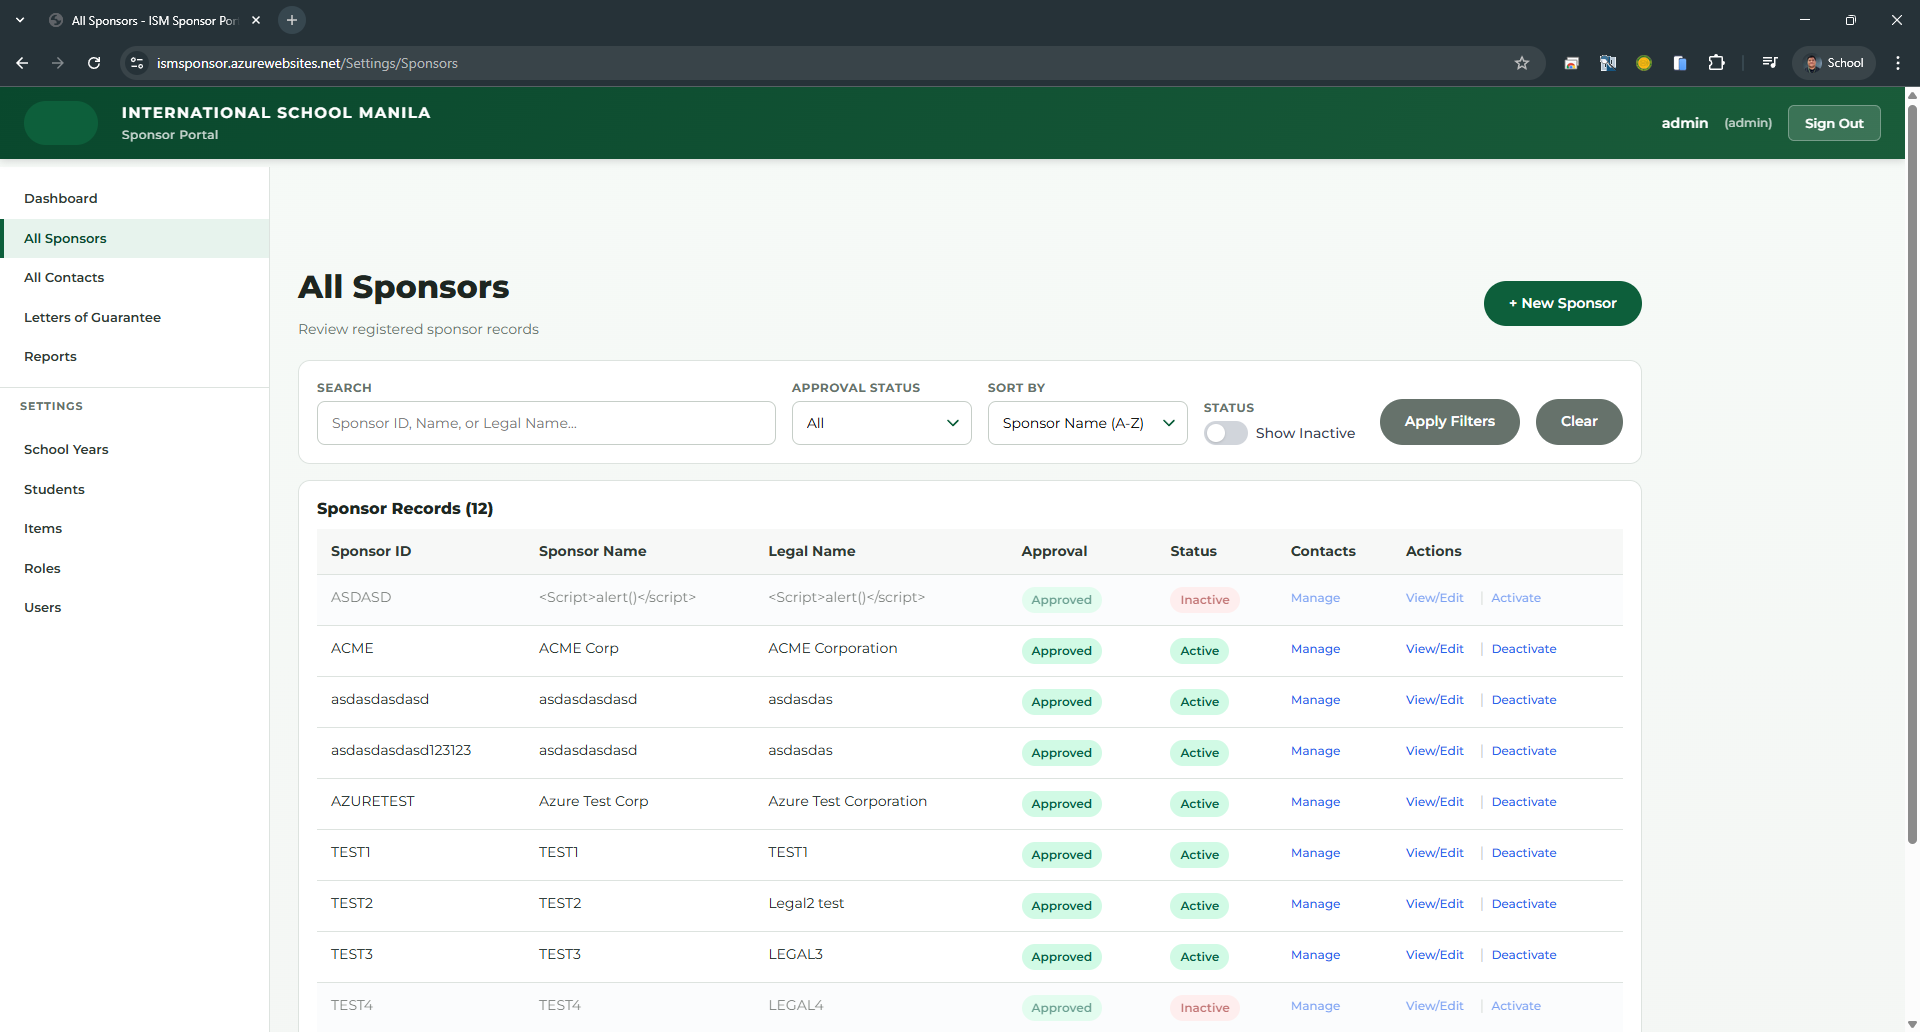
\includegraphics[width=0.90\linewidth]{images/current-interface/admin_all_sponsors.png}
        \caption{All Sponsors page for internal sponsor record management}
        \label{fig:current-all-sponsors}
    \end{figure}
    
    \noindent Figure~\ref{fig:current-all-sponsors} details the internal All Sponsors page, where staff can search, review, and maintain canonical sponsor records. The figure is included to show how the Sponsor Master reduces inconsistent sponsor naming and supports controlled sponsor record management.

    \begin{figure}[H]
        \centering
        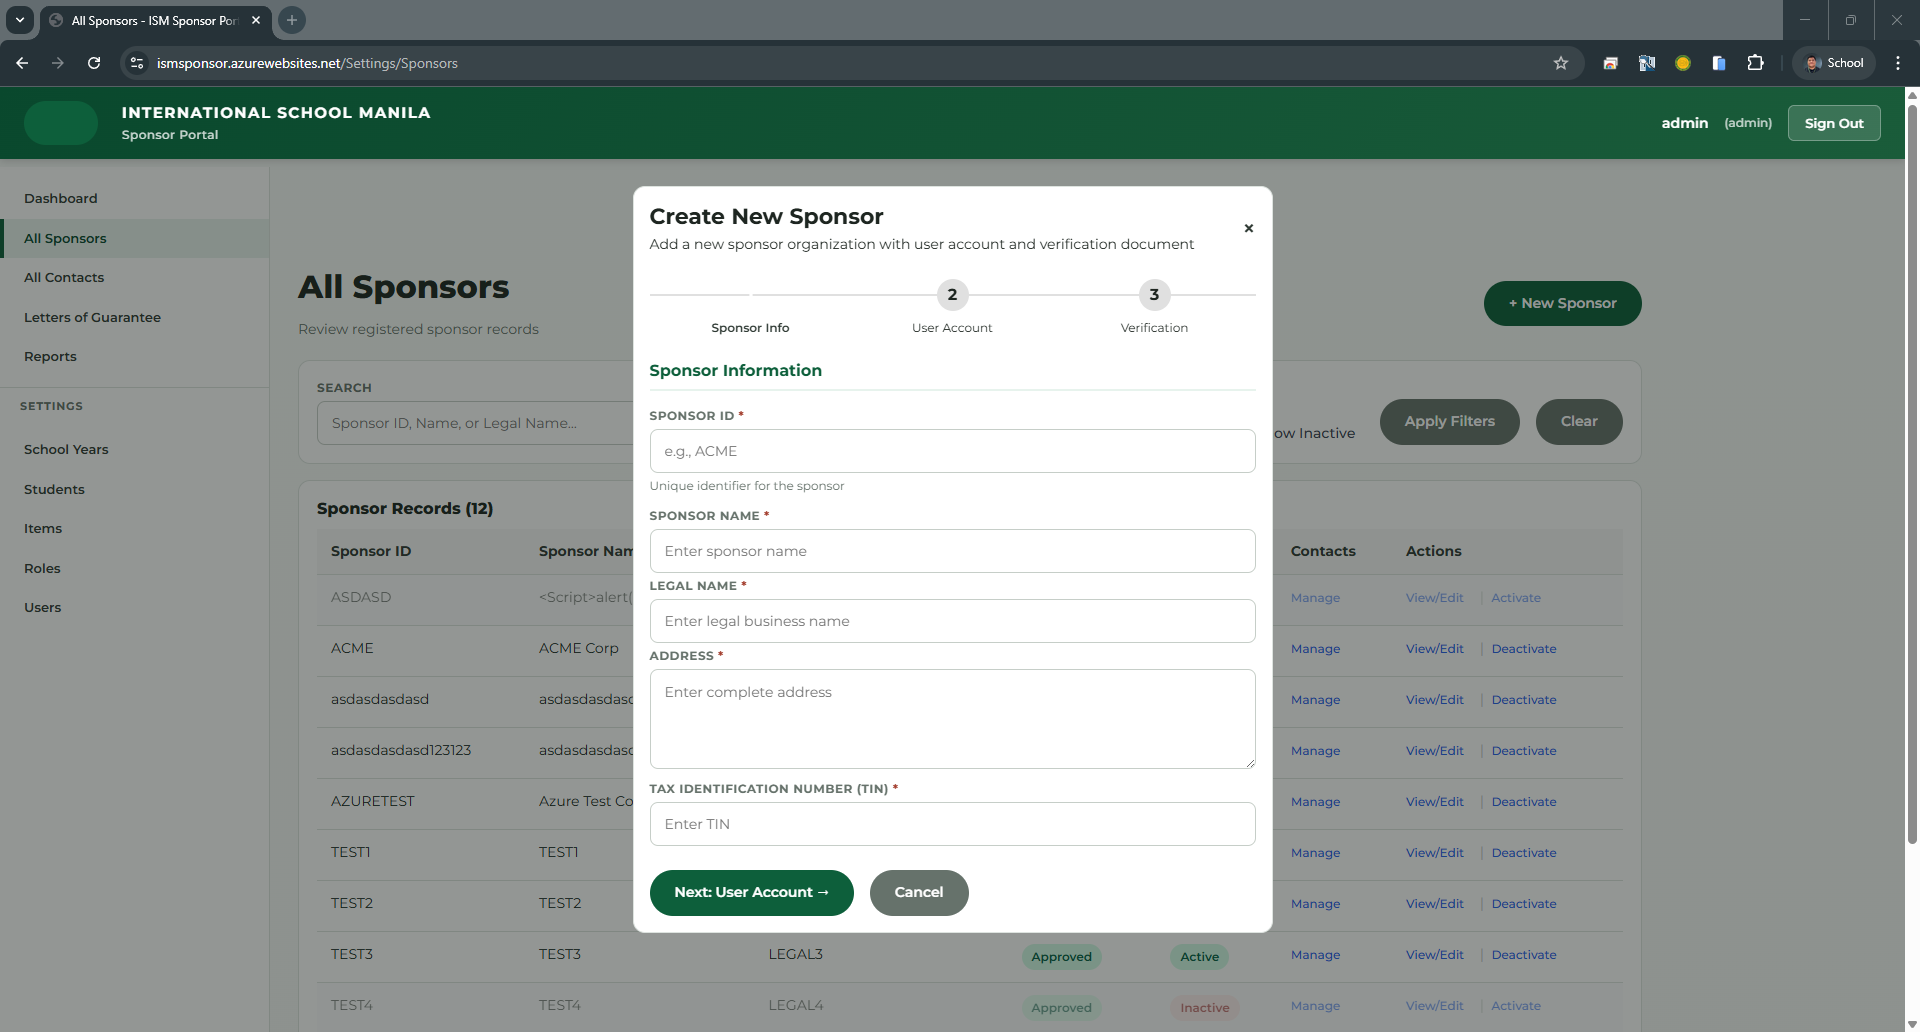
\includegraphics[width=0.90\linewidth]{images/current-interface/admin_create_sponsor.png}
        \caption{Create Sponsor page in the current Administrator interface}
        \label{fig:current-create-sponsor}
    \end{figure}

    \noindent Figure~\ref{fig:current-create-sponsor} details the Create Sponsor page, where administrator users enter sponsor identity, TIN, address, contact, and account-provisioning information. The figure is included to show how the pilot captures sponsor master data in structured fields rather than through informal notes or spreadsheets.
    \clearpage
    
    \begin{figure}[H]
        \centering
        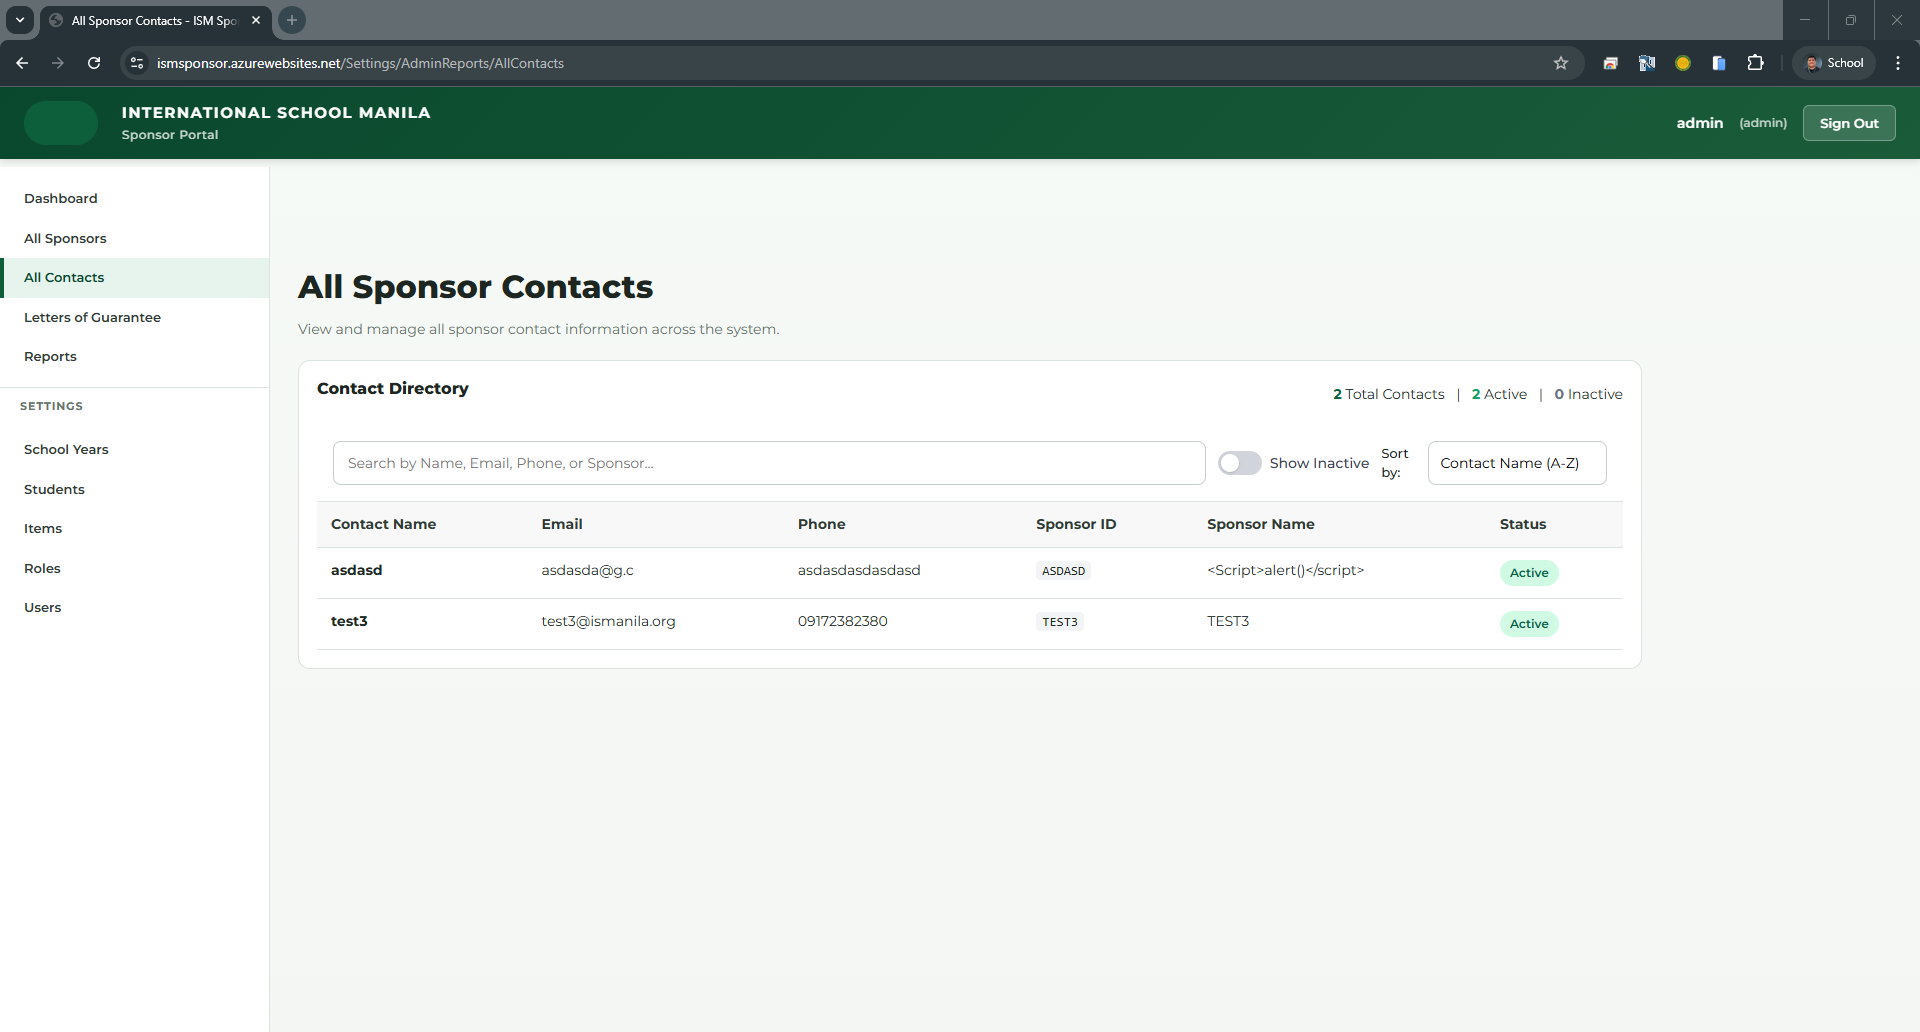
\includegraphics[width=0.90\linewidth]{images/current-interface/admin_all_contacts.png}
        \caption{All Contacts page for internal sponsor contact review}
        \label{fig:current-all-contacts}
    \end{figure}

    \noindent Figure~\ref{fig:current-all-contacts} details the All Contacts page used by staff to review sponsor contact records and related communication details. The figure is included to show how multiple sponsor contacts can be managed within the same controlled sponsor record.

    \begin{figure}[H]
        \centering
        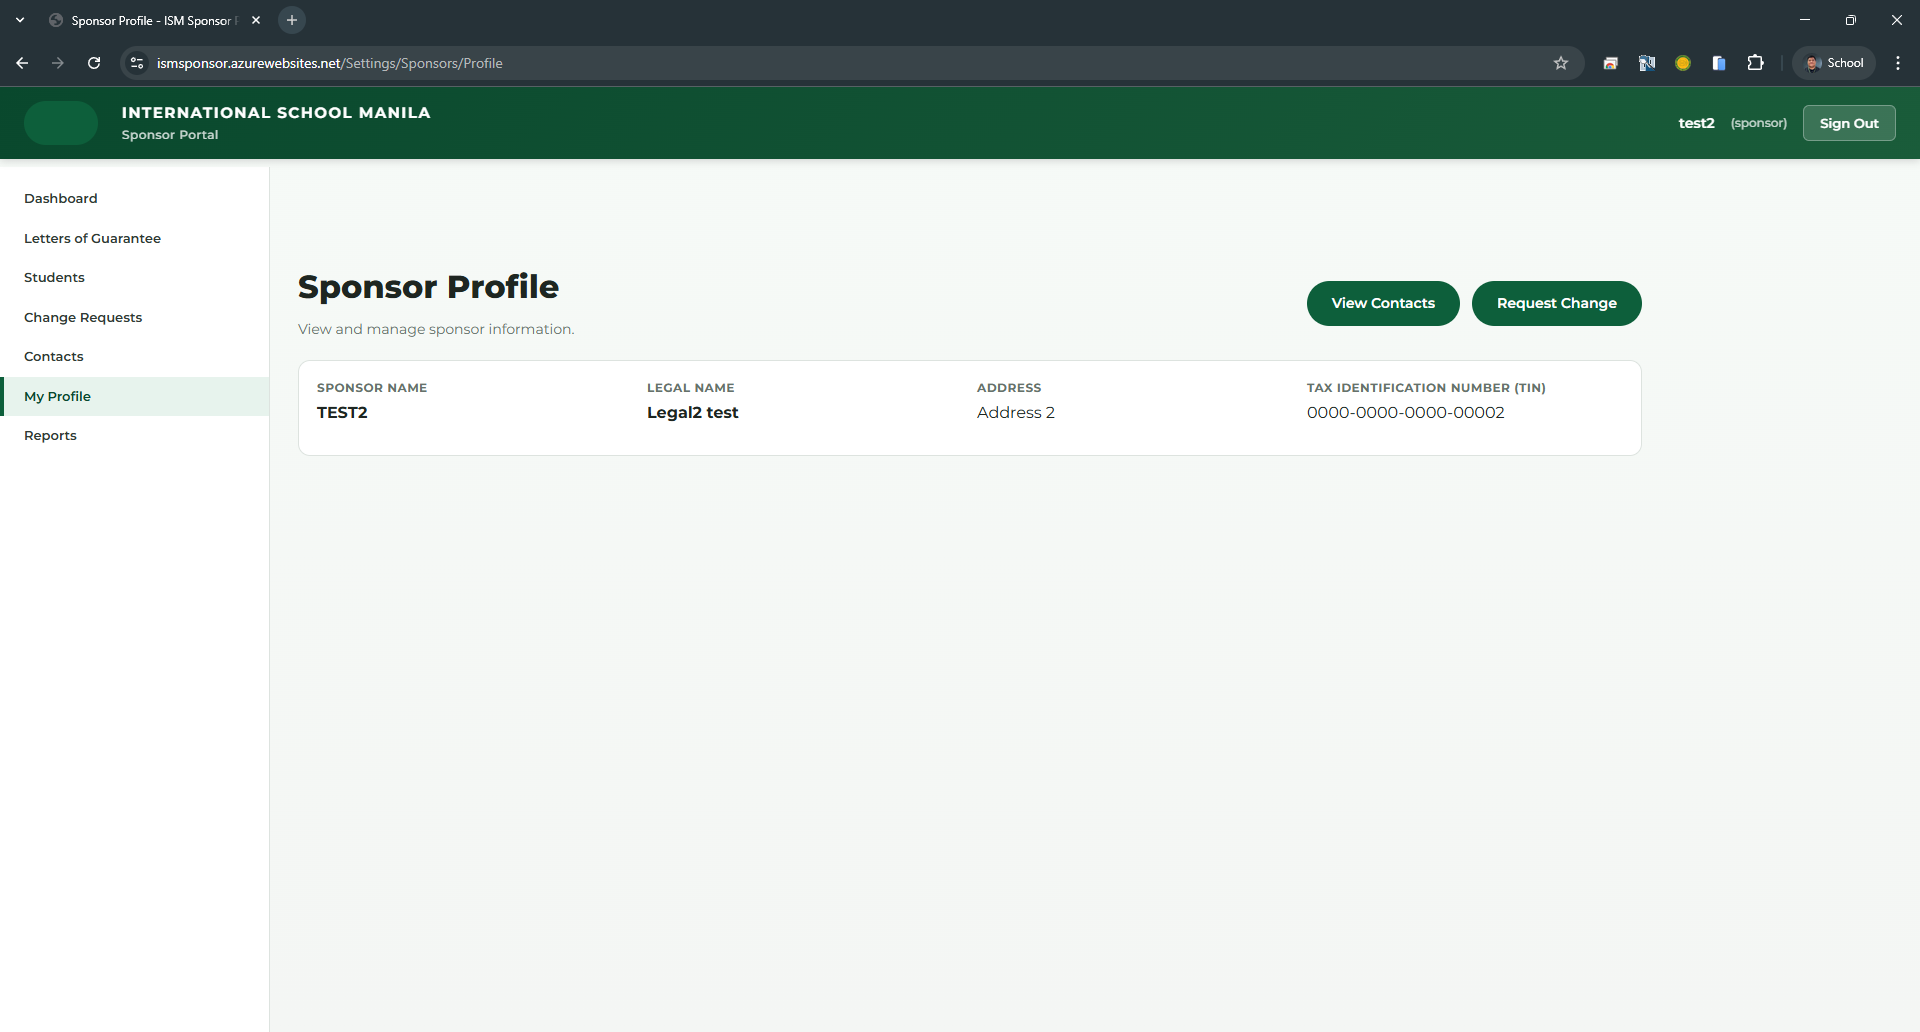
\includegraphics[width=0.90\linewidth]{images/current-interface/sponsor_profile.png}
        \caption{Sponsor profile page in the sponsor-facing portal}
        \label{fig:current-sponsor-profile}
    \end{figure}

    \noindent Figure~\ref{fig:current-sponsor-profile} details the sponsor-facing profile page, where external sponsor users can view their own approved organization information. The figure is included to show how sponsor self-service improves transparency while preventing direct uncontrolled edits to the Sponsor Master.

    \begin{figure}[H]
        \centering
        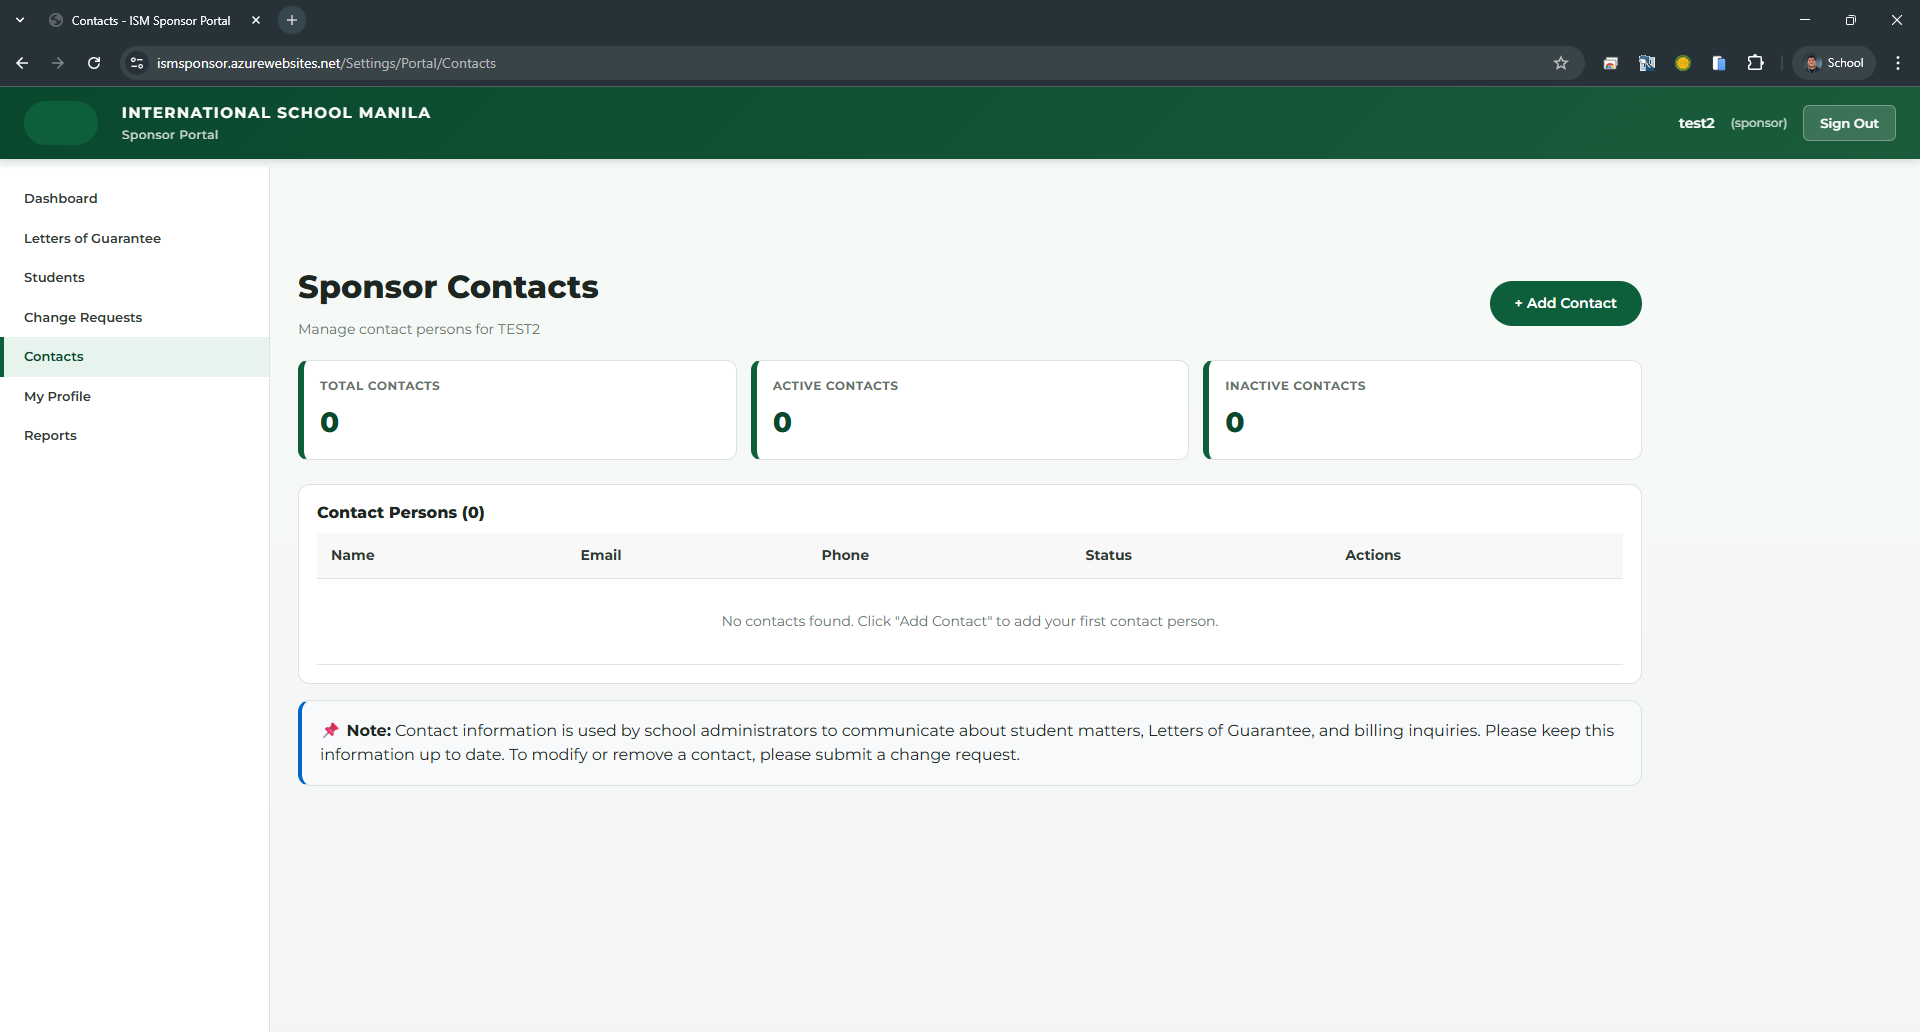
\includegraphics[width=0.90\linewidth]{images/current-interface/sponsor_contacts.png}
        \caption{Sponsor contacts page in the sponsor-facing portal}
        \label{fig:current-sponsor-contacts}
    \end{figure}

    \noindent Figure~\ref{fig:current-sponsor-contacts} details the sponsor-facing contacts page, where sponsor users can view contact information associated with their organization. The figure is included to show how external users can verify contact records without seeing records that belong to other sponsors.
    \clearpage

    \subsubsection{Letters of Guarantee and Coverage Views}
    
    Letters of Guarantee are put in place via internal and sponsor facing views. The Letters of Guarantee page is for internal users to view LoG records, develop LoGs, manage LoG coverage rules and verify LoG information. The sponsor user can see the assigned Letters of Guarantee from the sponsor portal but only in their records.

    \begin{figure}[H]
        \centering
        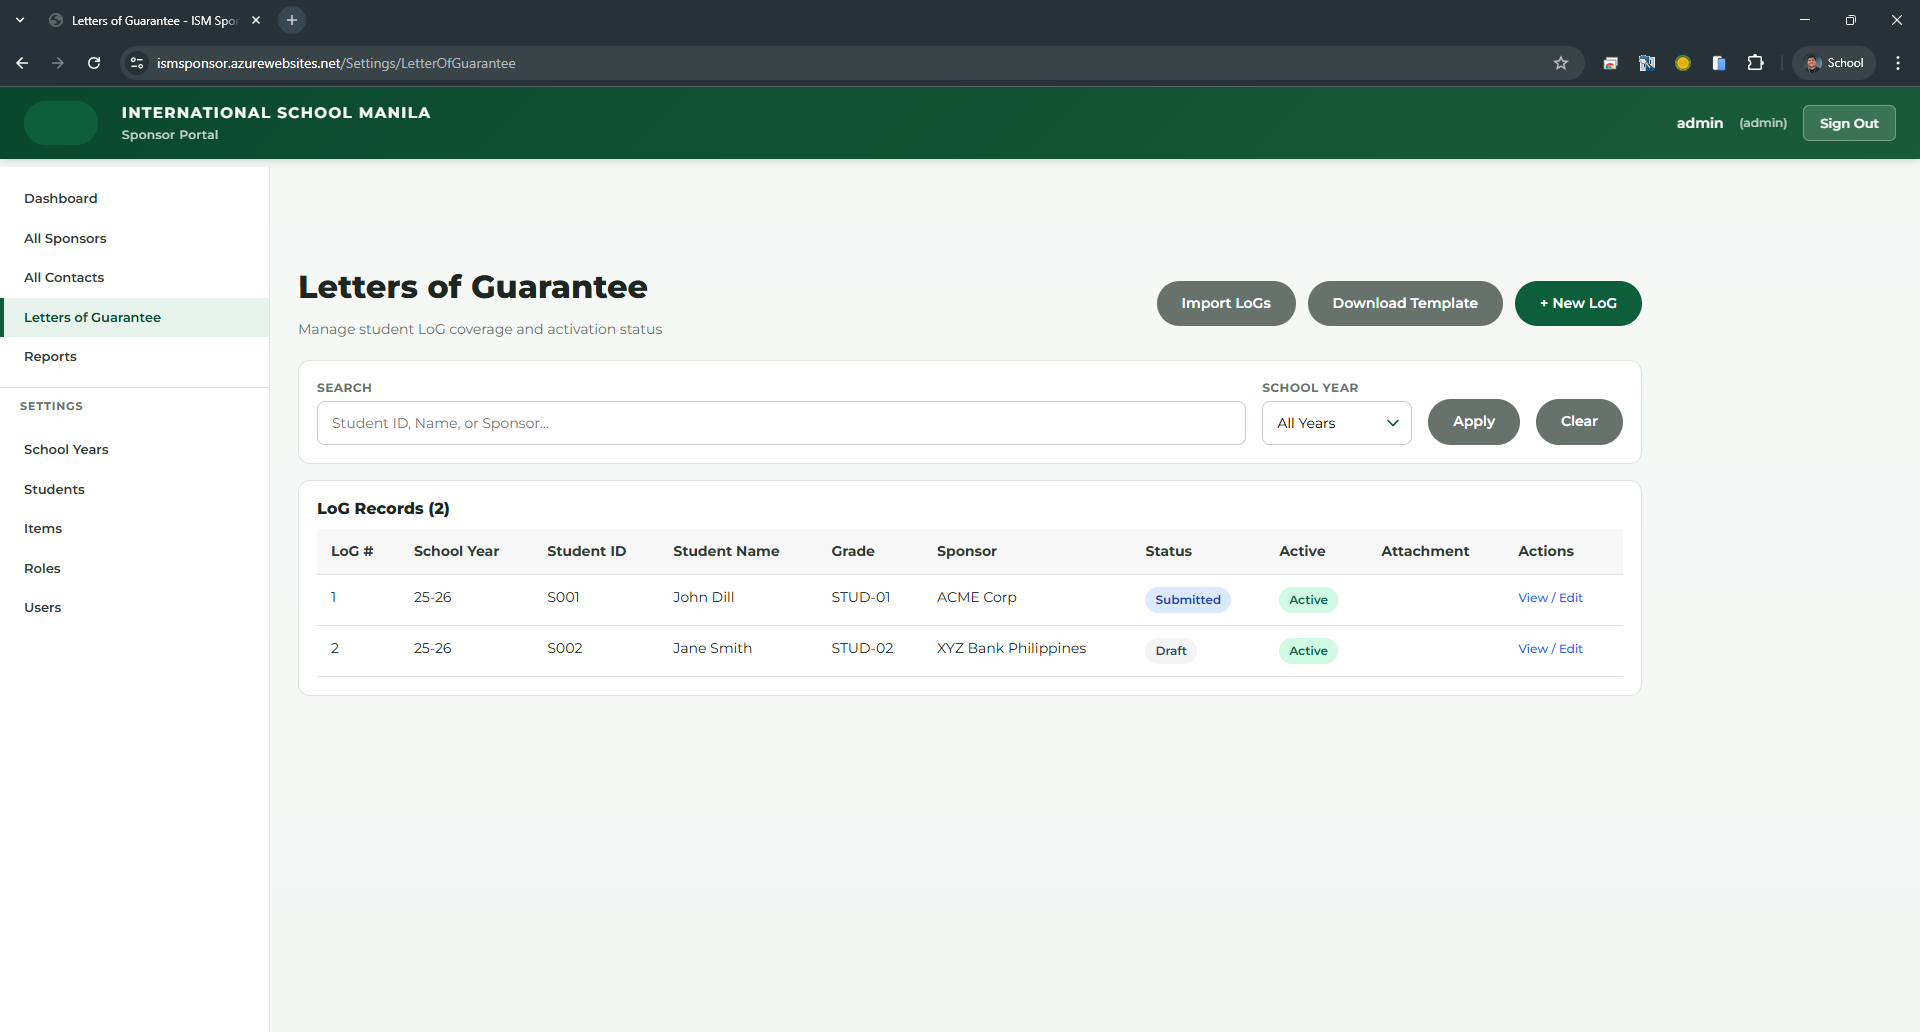
\includegraphics[width=0.90\linewidth]{images/current-interface/admin_log_list.png}
        \caption{Letters of Guarantee page for internal users}
        \label{fig:current-log-list}
    \end{figure}

    \noindent Figure~\ref{fig:current-log-list} details the internal Letters of Guarantee list used by staff to review LoG records, status values, attachments, and coverage actions. The figure is included to show how LoG records are made visible as structured workflow items rather than separate manually interpreted documents.

    \begin{figure}[H]
        \centering
        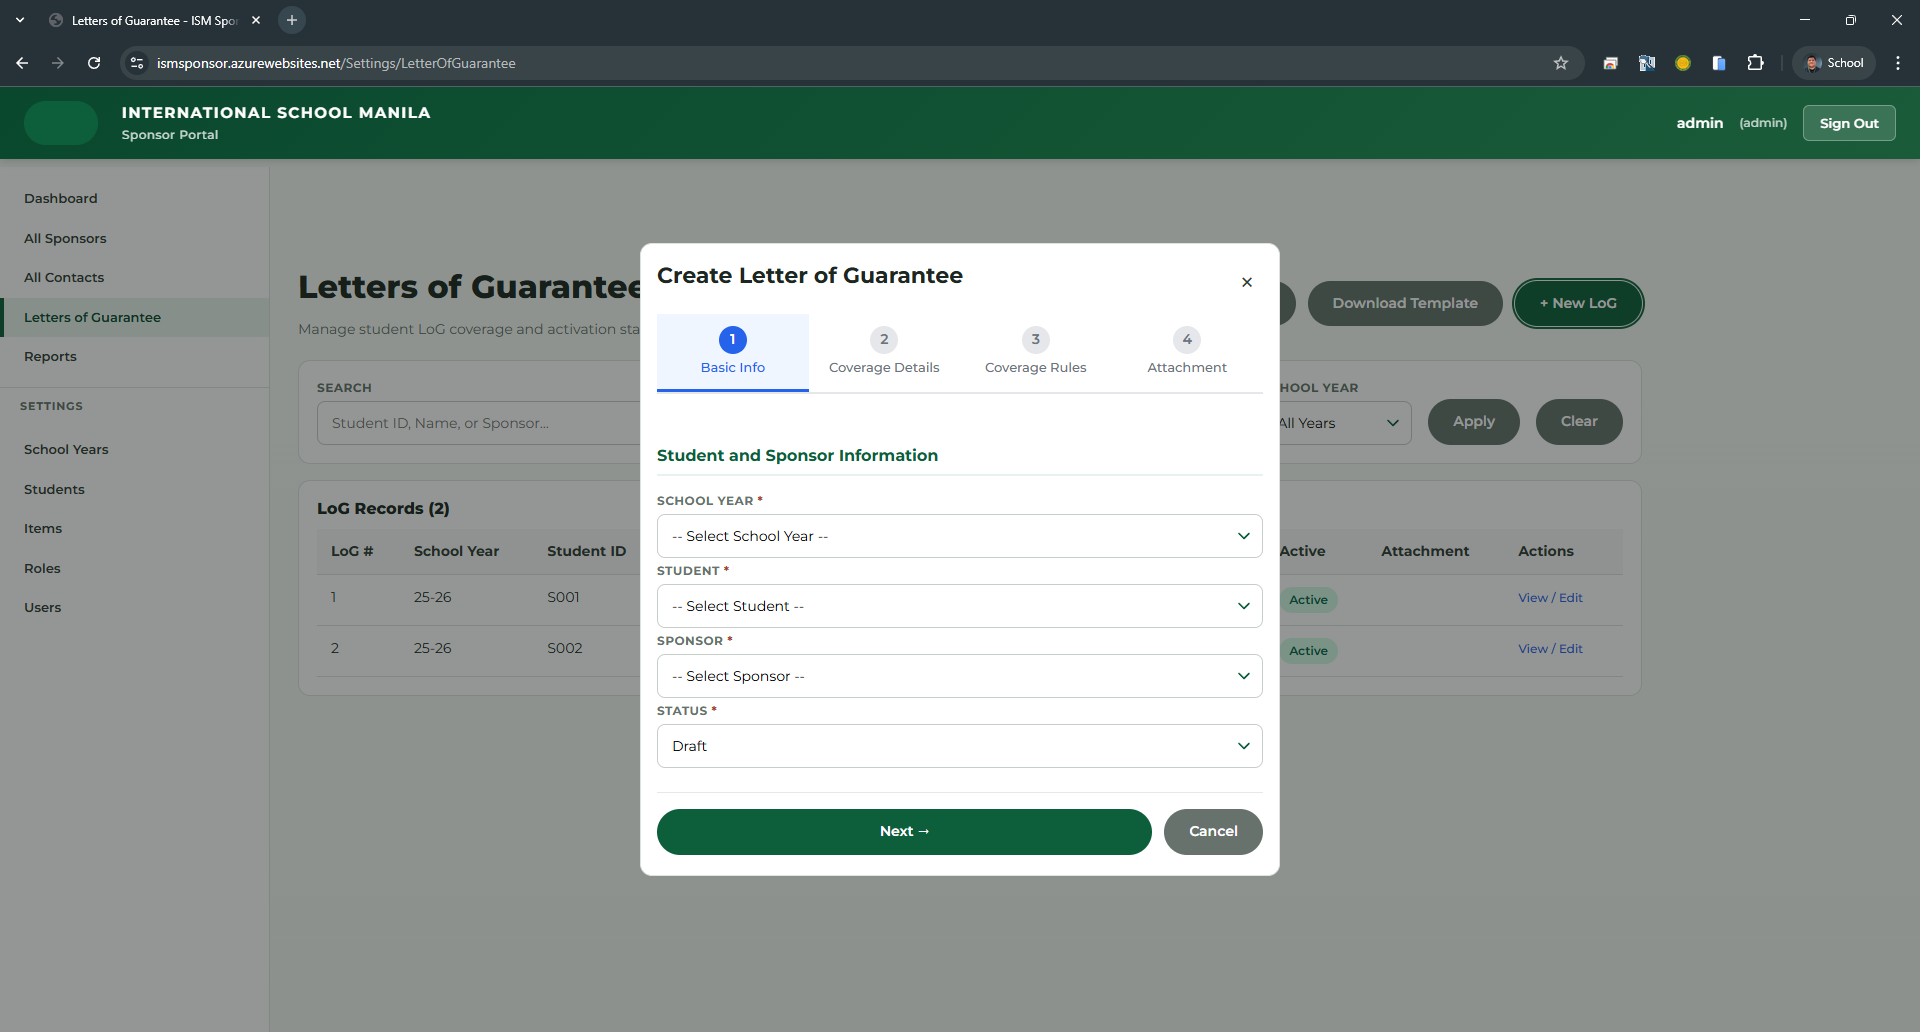
\includegraphics[width=0.90\linewidth]{images/current-interface/admin_create_log.png}
        \caption{Create Letter of Guarantee page with coverage-related fields}
        \label{fig:current-create-log}
    \end{figure}

    \noindent Figure~\ref{fig:current-create-log} details the LoG creation form, where staff define student, sponsor, school year, effective dates, status, and coverage-related fields. The figure is included to show how LoG content is converted into rule-ready data for later coverage evaluation.

    \begin{figure}[H]
        \centering
        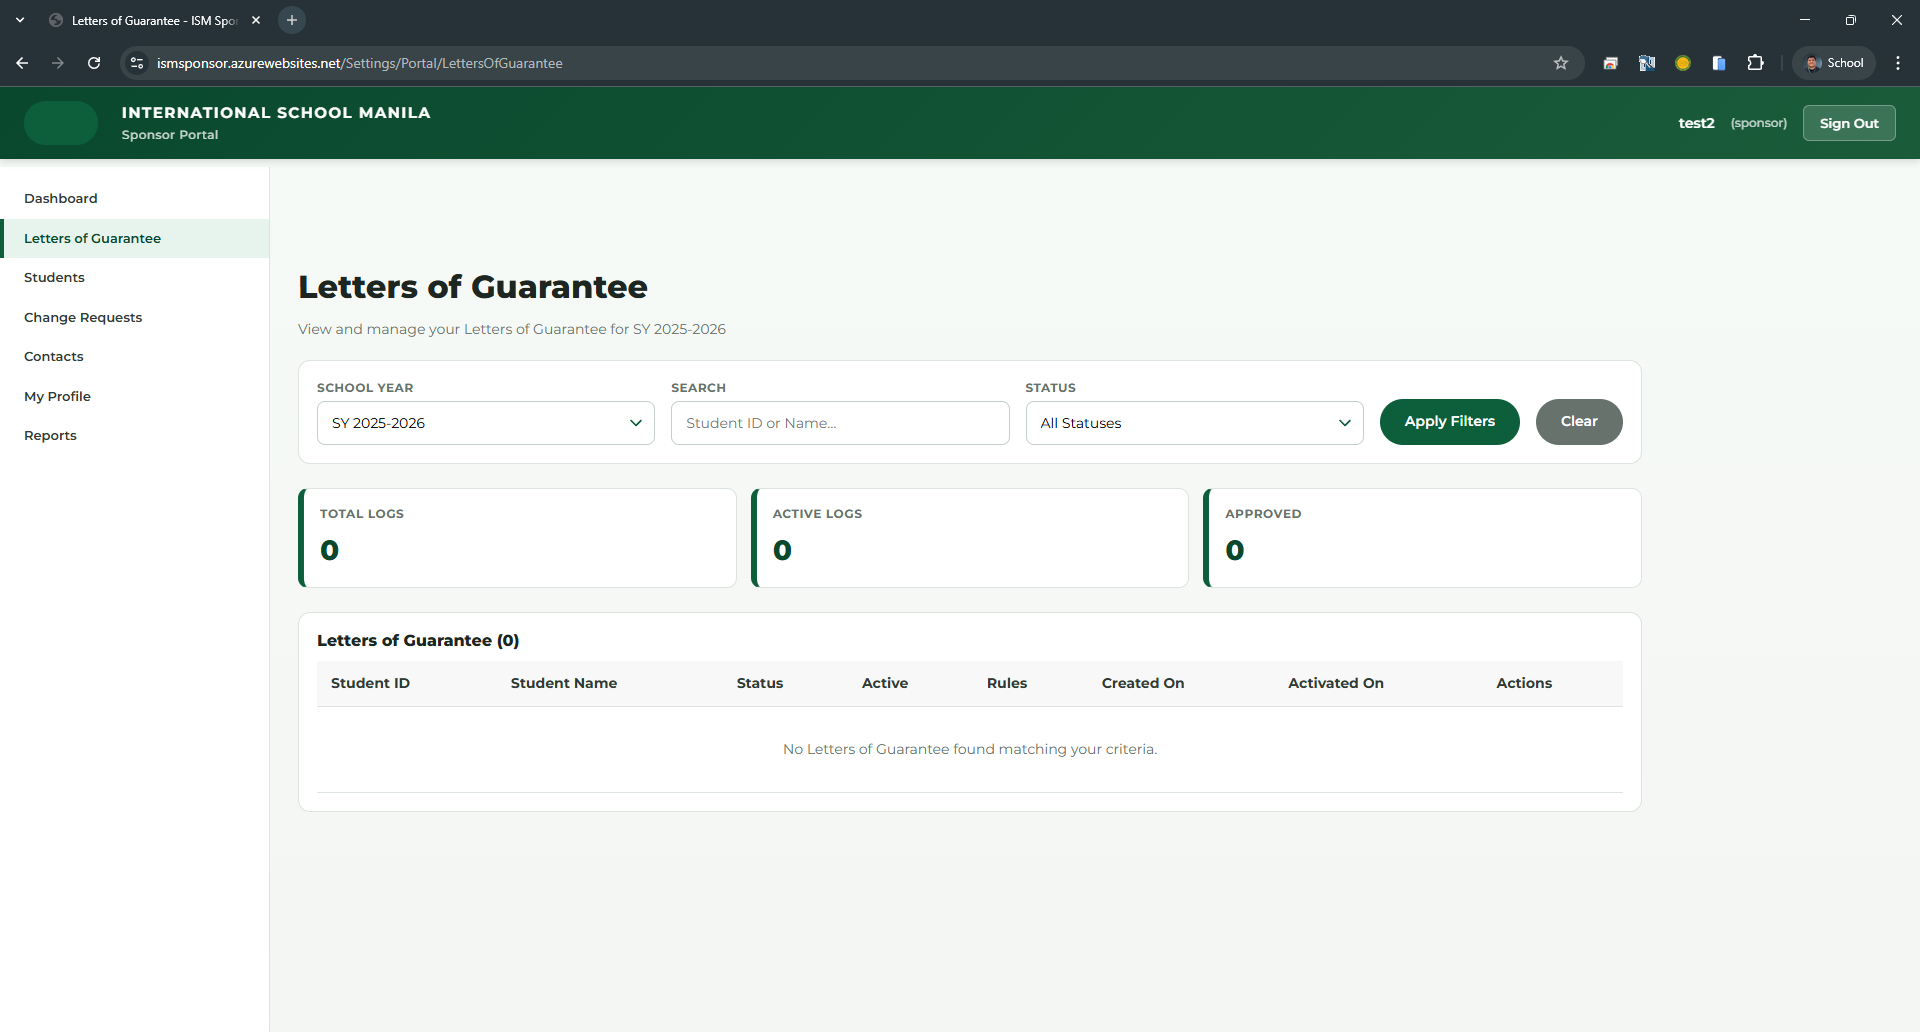
\includegraphics[width=0.90\linewidth]{images/current-interface/sponsor_logs.png}
        \caption{Sponsor-facing Letters of Guarantee page}
        \label{fig:current-sponsor-logs}
    \end{figure}

    \noindent Figure~\ref{fig:current-sponsor-logs} details the sponsor-facing LoG page, where sponsor users can review only the LoG records associated with their own organization. The figure is included to show how the pilot provides sponsor visibility without exposing internal administrative functions.

    \begin{figure}[H]
        \centering
        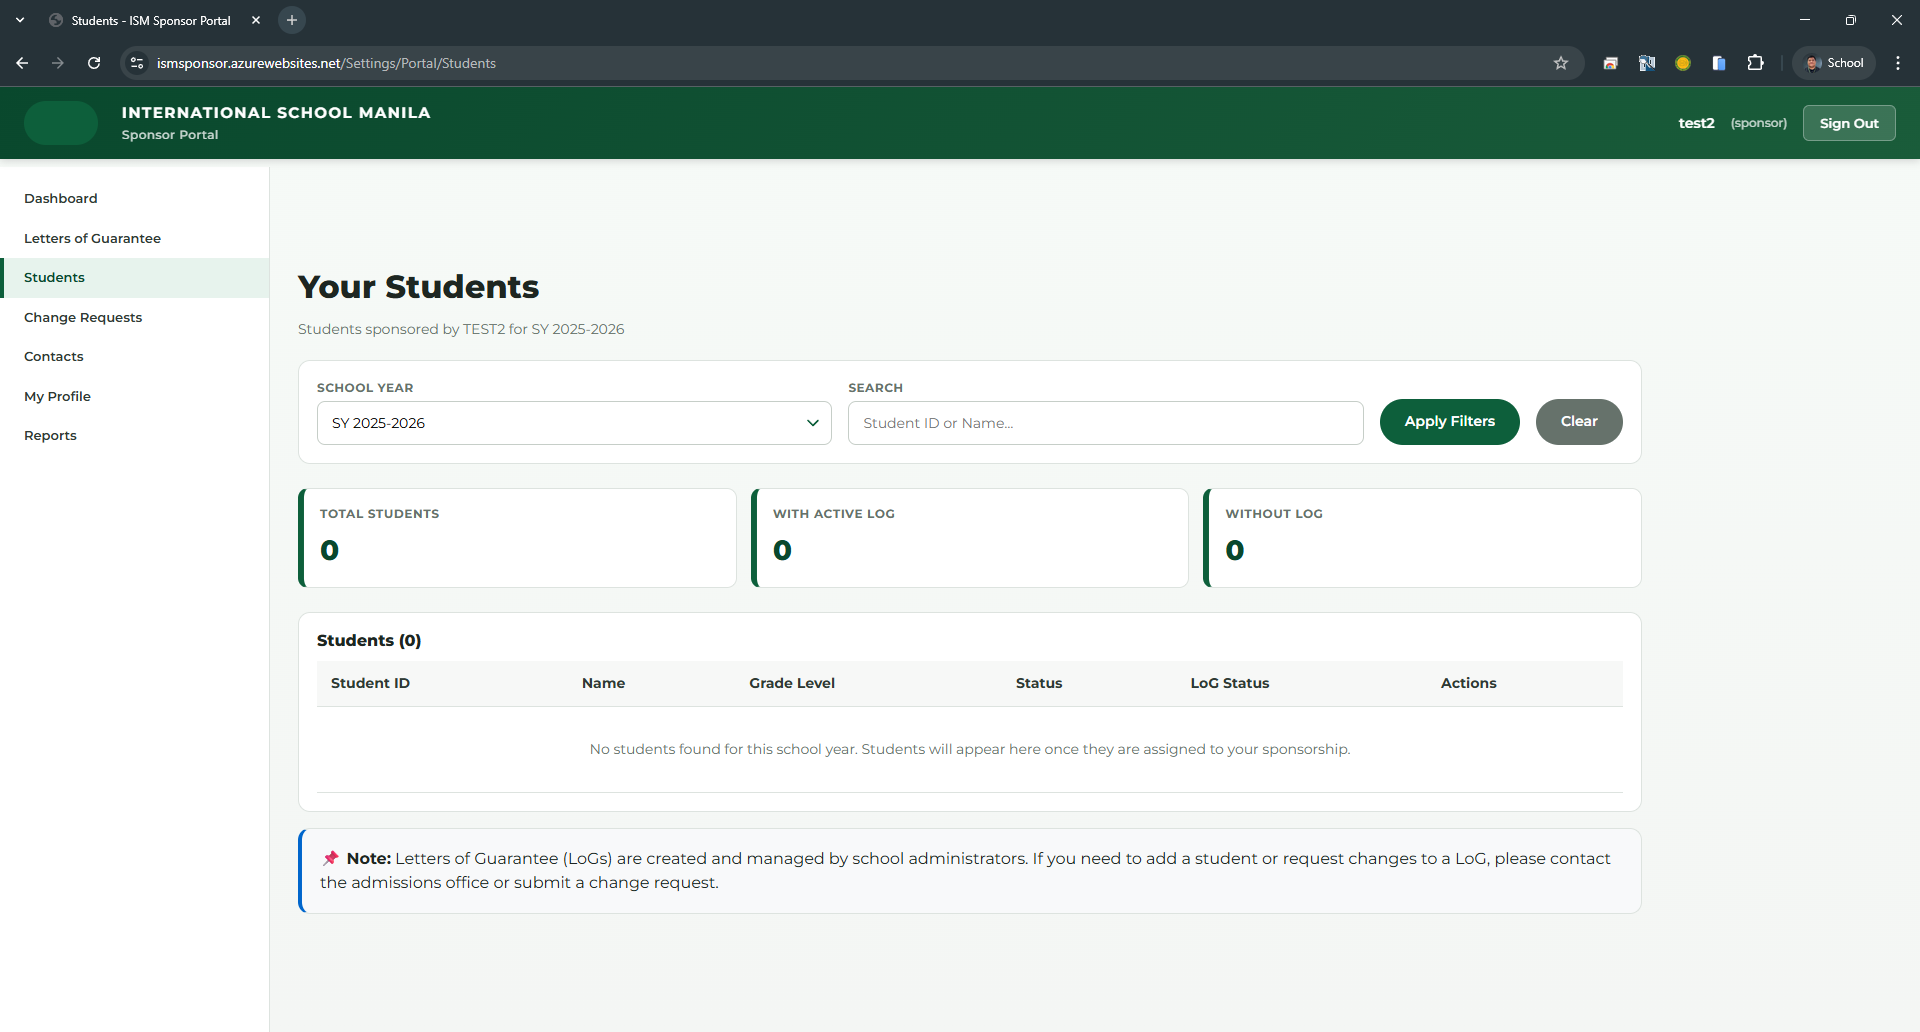
\includegraphics[width=0.90\linewidth]{images/current-interface/sponsor_students.png}
        \caption{Sponsor-facing Students page showing assigned students}
        \label{fig:current-sponsor-students}
    \end{figure}

    \noindent Figure~\ref{fig:current-sponsor-students} details the sponsor-facing Students page, where sponsor users can view students linked to their sponsor account within the permitted scope. The figure is included to show how sponsor-student relationships are presented as controlled records rather than informal references.
    \clearpage

    \subsubsection{Change Requests and Sponsor Self-Service}
    
    The deployed pilot comes with sponsor self-service option to submit and review change requests. These screens minimize the informal handling of update and help manage the governance process that sponsor profile updates are to be reviewed prior to making changes to sponsor master.

    \begin{figure}[H]
        \centering
        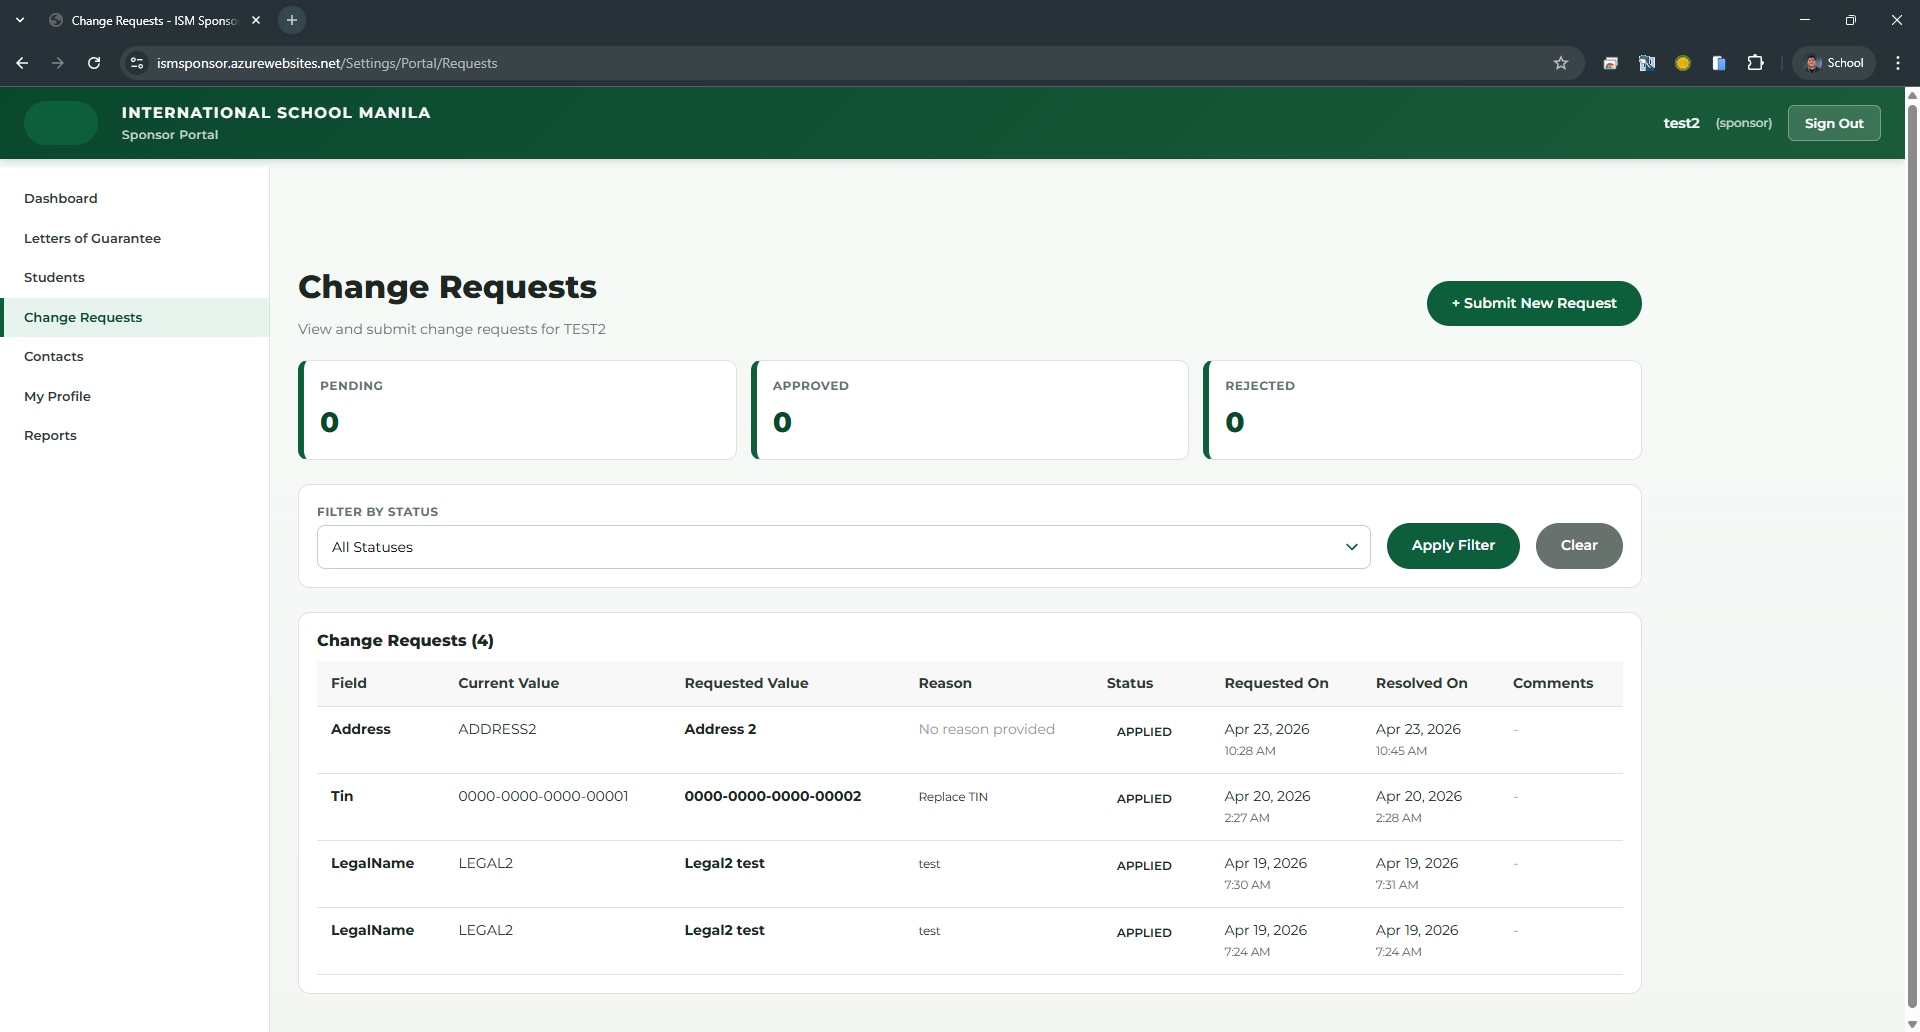
\includegraphics[width=0.90\linewidth]{images/current-interface/sponsor_change_requests.png}
        \caption{Sponsor change requests page in the sponsor-facing portal}
        \label{fig:current-sponsor-change-requests}
    \end{figure}

    \noindent Figure~\ref{fig:current-sponsor-change-requests} details the sponsor change-request page, where sponsors can submit and monitor requested updates to controlled profile information. The figure is included to show how the portal supports sponsor self-service while preserving staff review before changes affect the Sponsor Master.

    \begin{figure}[H]
        \centering
        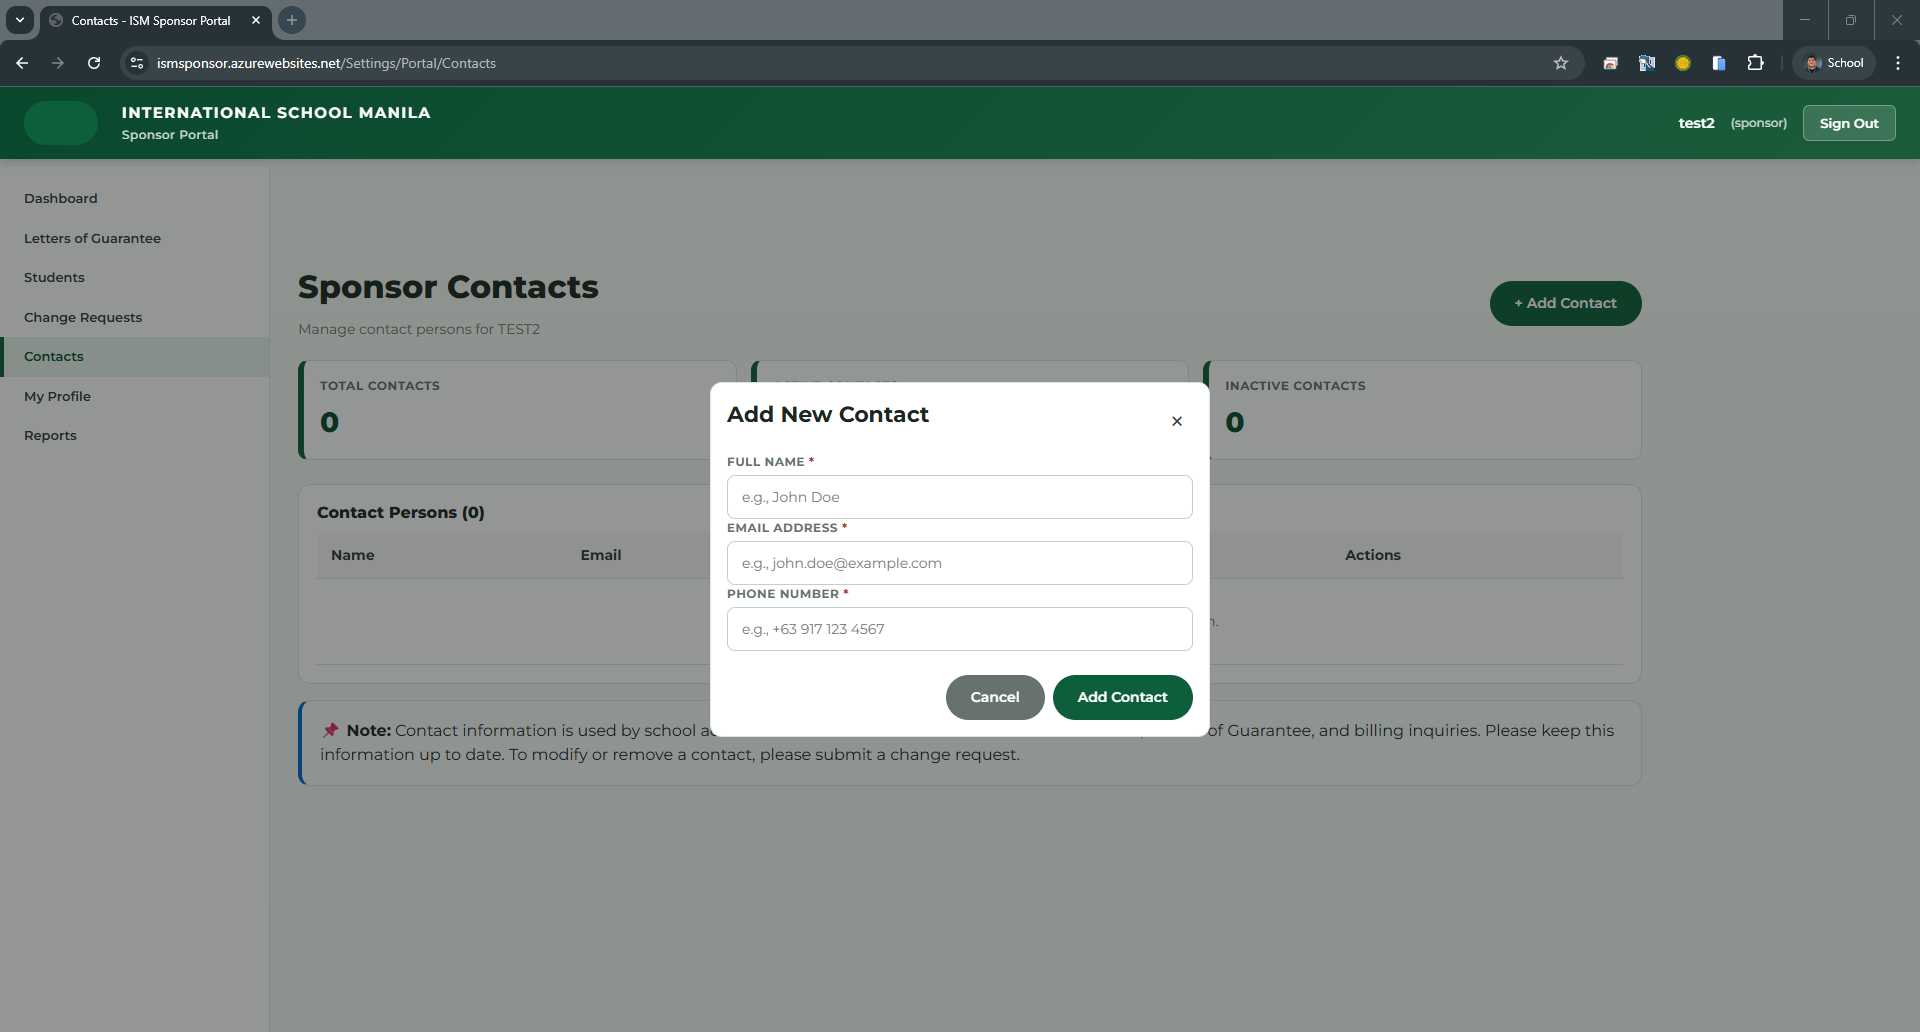
\includegraphics[width=0.90\linewidth]{images/current-interface/sponsor_add_contact.png}
        \caption{Add New Contact page for sponsor self-service updates}
        \label{fig:current-sponsor-add-contact}
    \end{figure}

    \noindent Figure~\ref{fig:current-sponsor-add-contact} details the sponsor self-service contact form, which allows a sponsor to request or add contact information through a controlled workflow. The figure is included to show how contact updates can be captured in structured form instead of being handled only through email or manual follow-up.
    \clearpage
    % FORMAT HIGHLIGHT: subsubsection heading
    % FORMAT HIGHLIGHT: LaTeX-safe conversion only; source wording retained
    
    \subsubsection{Reports and Monitoring Views}
    
    There is a role-aware Reports page in the deployed pilot. Administrative users will have access to administrative and monitoring reports, and Sponsor users will have access to reports for their own LoG and their students. This separation of report based on role helps the operational review without revealing information outside the boundary of each user's permission.
    
    \setlength{\LTleft}{0pt}
    \setlength{\LTright}{\fill}
    \begin{longtable}{>{\raggedright\arraybackslash}p{0.20\linewidth}
            >{\raggedright\arraybackslash}p{0.72\linewidth}}
    \caption{Implemented report access by role}\label{table:implemented-report-access}\\
    \toprule
    \textbf{Role} & \textbf{Reports available in the deployed pilot} \\
    \midrule
    \endfirsthead
    \caption[]{Implemented report access by role (continued)}\\
    \toprule
    \textbf{Role} & \textbf{Reports available in the deployed pilot} \\
    \midrule
    \endhead
    \midrule
    \multicolumn{2}{r}{\textit{Continued on next page}}\\
    \endfoot
    \bottomrule
    \endlastfoot
    \textbf{Administrator} & LoG Activity; Coverage Decisions; Sponsor Master; Sync Status; Audit Activity; Coverage Rules; Reconciliation Report; Coverage Tracking. \\
            \textbf{Admissions} & Coverage Tracking. \\
            \textbf{Cashier} & Reconciliation Report. \\
            \textbf{Sponsor} & My Letters of Guarantee; My Students. \\
    \end{longtable}

    Table~\ref{table:implemented-report-access} is placed before the report screenshots so the reader can first see the report permissions, then visually confirm how report access appears in the interface. Figure~\ref{fig:current-admin-reports} documents the staff-facing administrative reports page, while Figure~\ref{fig:current-sponsor-reports} documents the sponsor-facing reports page limited to sponsor-specific outputs.

    \begin{figure}[H]
        \centering
        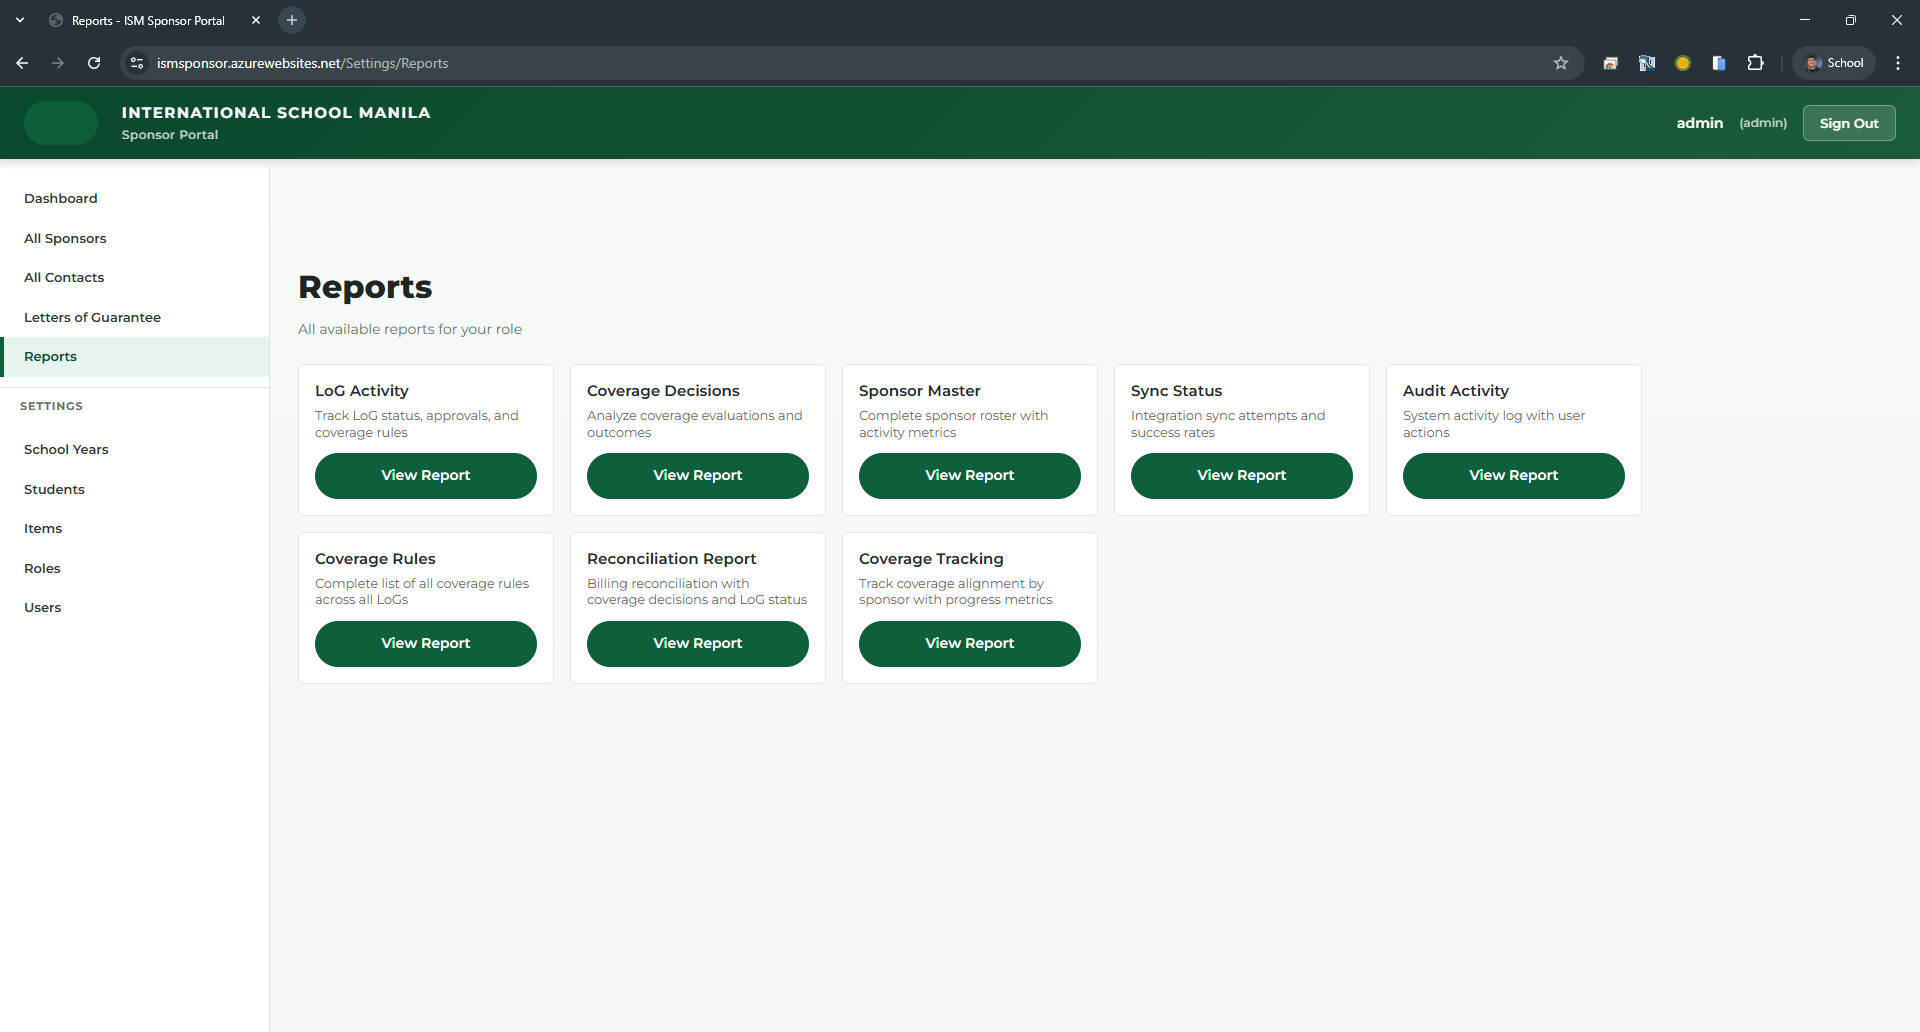
\includegraphics[width=0.90\linewidth]{images/current-interface/admin_reports.png}
        \caption{Administrator reports page in the current deployed pilot web application}
        \label{fig:current-admin-reports}
    \end{figure}

    \noindent Figure~\ref{fig:current-admin-reports} details the Administrator reports page, where staff can access administrative, audit, coverage, reconciliation, and monitoring-related reports. The figure is included to show how the pilot supports internal review of sponsor records, coverage decisions, and operational activity.

    \begin{figure}[H]
        \centering
        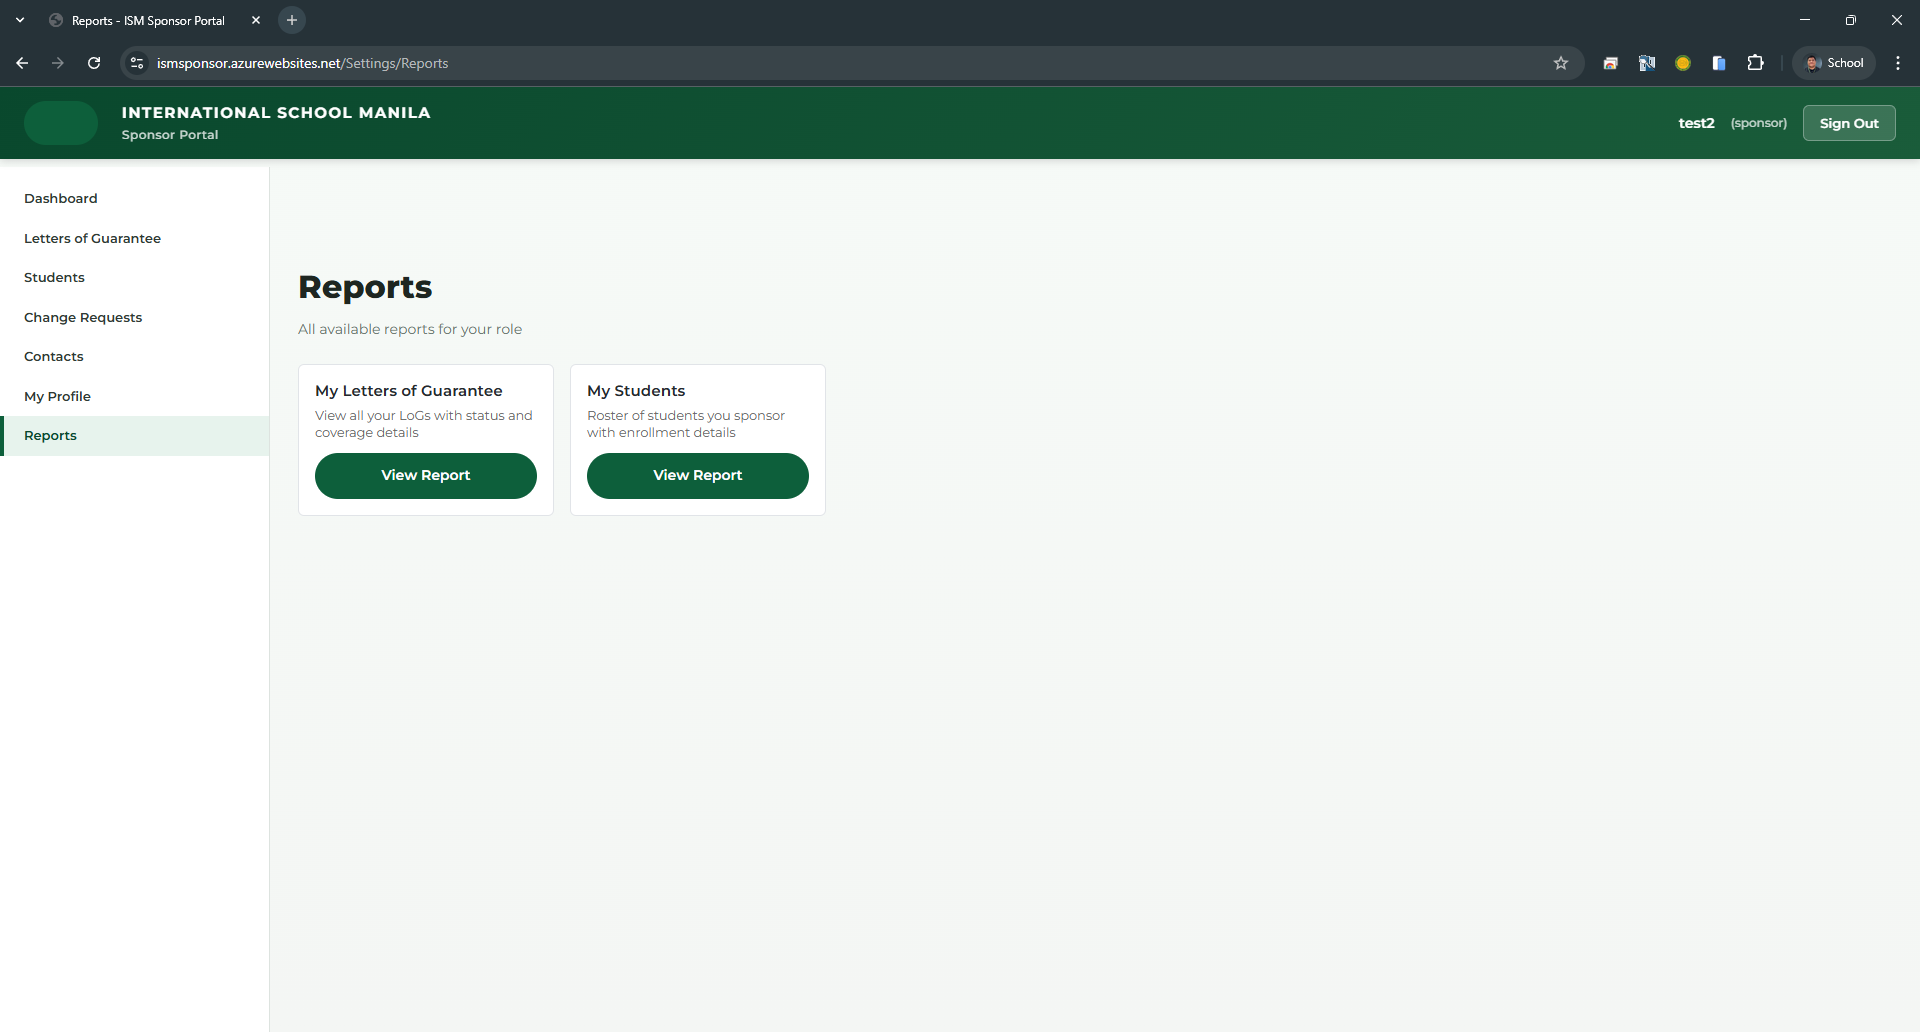
\includegraphics[width=0.90\linewidth]{images/current-interface/sponsor_reports.png}
        \caption{Sponsor reports page in the sponsor-facing portal}
        \label{fig:current-sponsor-reports}
    \end{figure}

    \noindent Figure~\ref{fig:current-sponsor-reports} details the sponsor-facing reports page, where report access is limited to sponsor-specific LoG and student outputs. The figure is included to show how reporting is separated by role so that external sponsors can review their own records without accessing institutional or other sponsor data.

    \subsubsection{Administrative Settings and Data Maintenance}
    
    Administrative settings are taken care of through unique pages for School Years, Students, Items, Roles, and Users. These pages store the reference data required for the pilot system to work. The records for school years create active periods, student records provide data for sponsors and status, item records provide data for coverage, role records control access, and user records provide data for user accounts.    

    \begin{figure}[H]
        \centering
        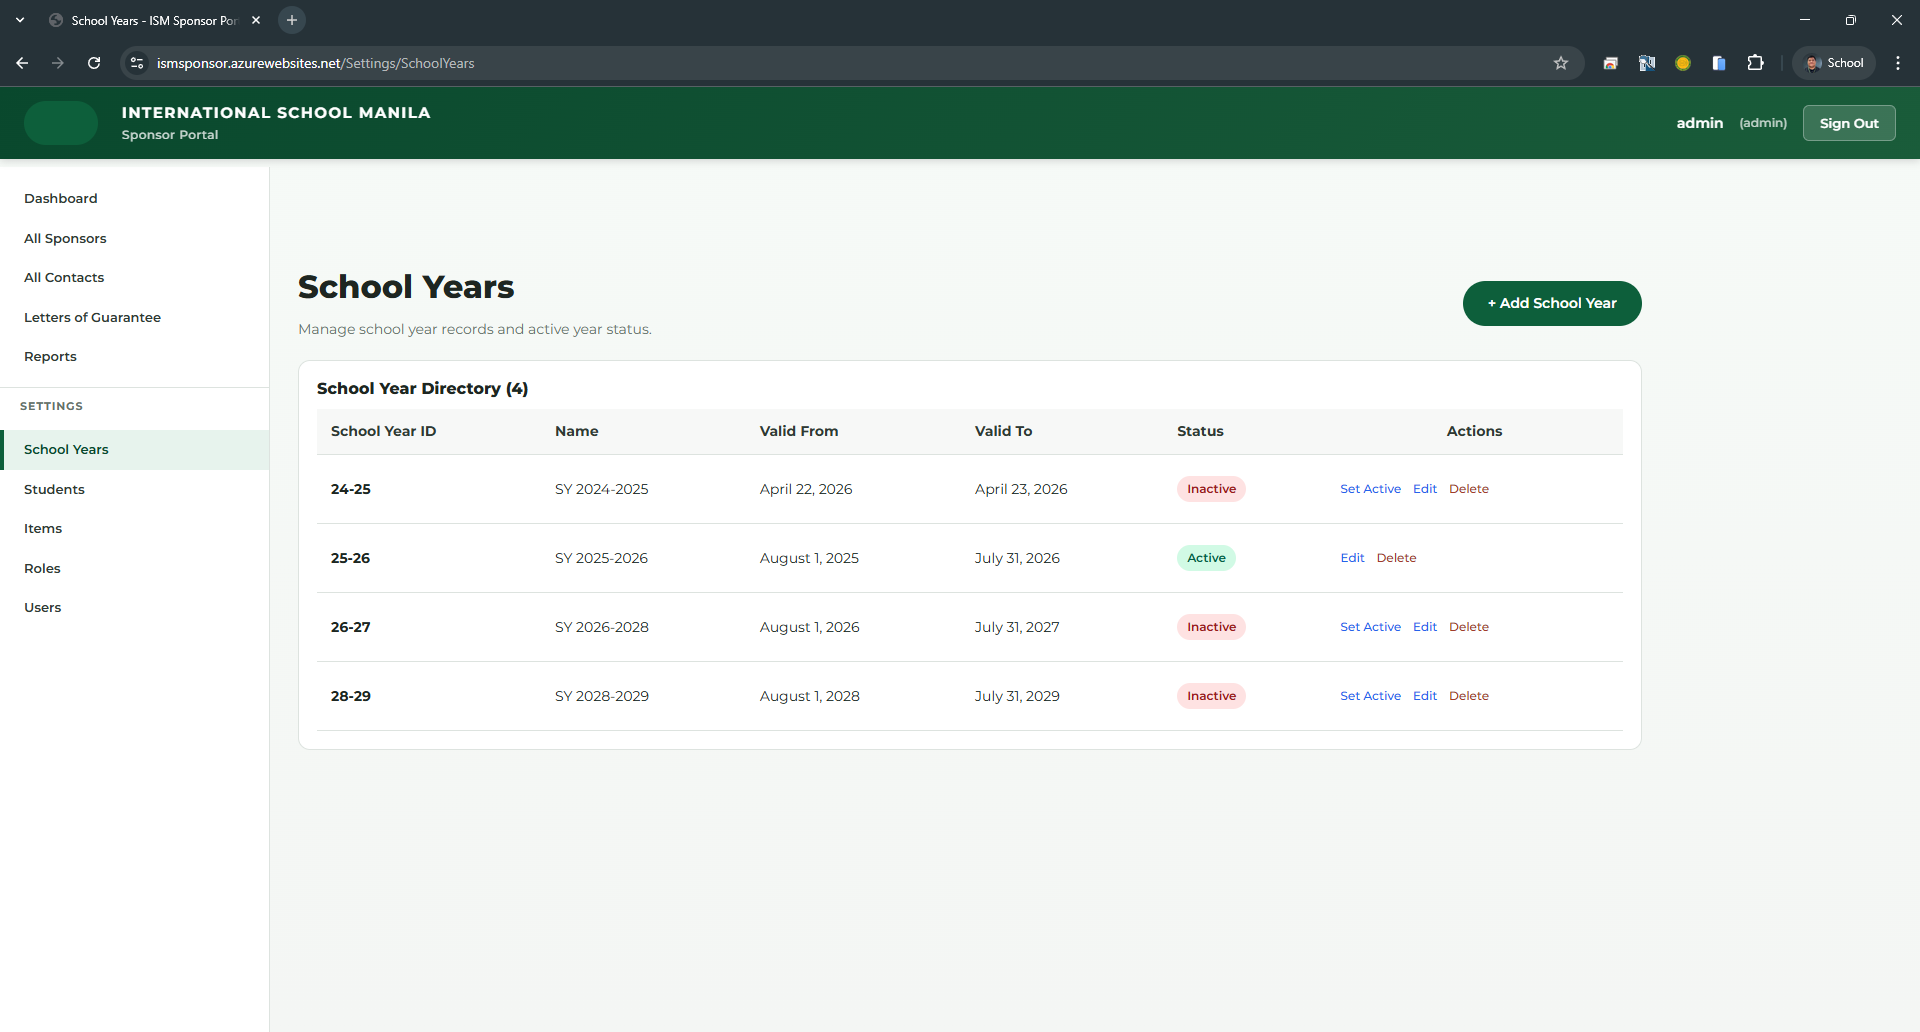
\includegraphics[width=0.90\linewidth]{images/current-interface/admin_school_years.png}
        \caption{School Years management page}
        \label{fig:current-school-years}
    \end{figure}

    \noindent Figure~\ref{fig:current-school-years} details the School Years management page, which maintains active periods used by dashboard, LoG, coverage, and reporting views. The figure is included to show how date-based coverage and reporting depend on controlled school-year reference data.

    \begin{figure}[H]
        \centering
        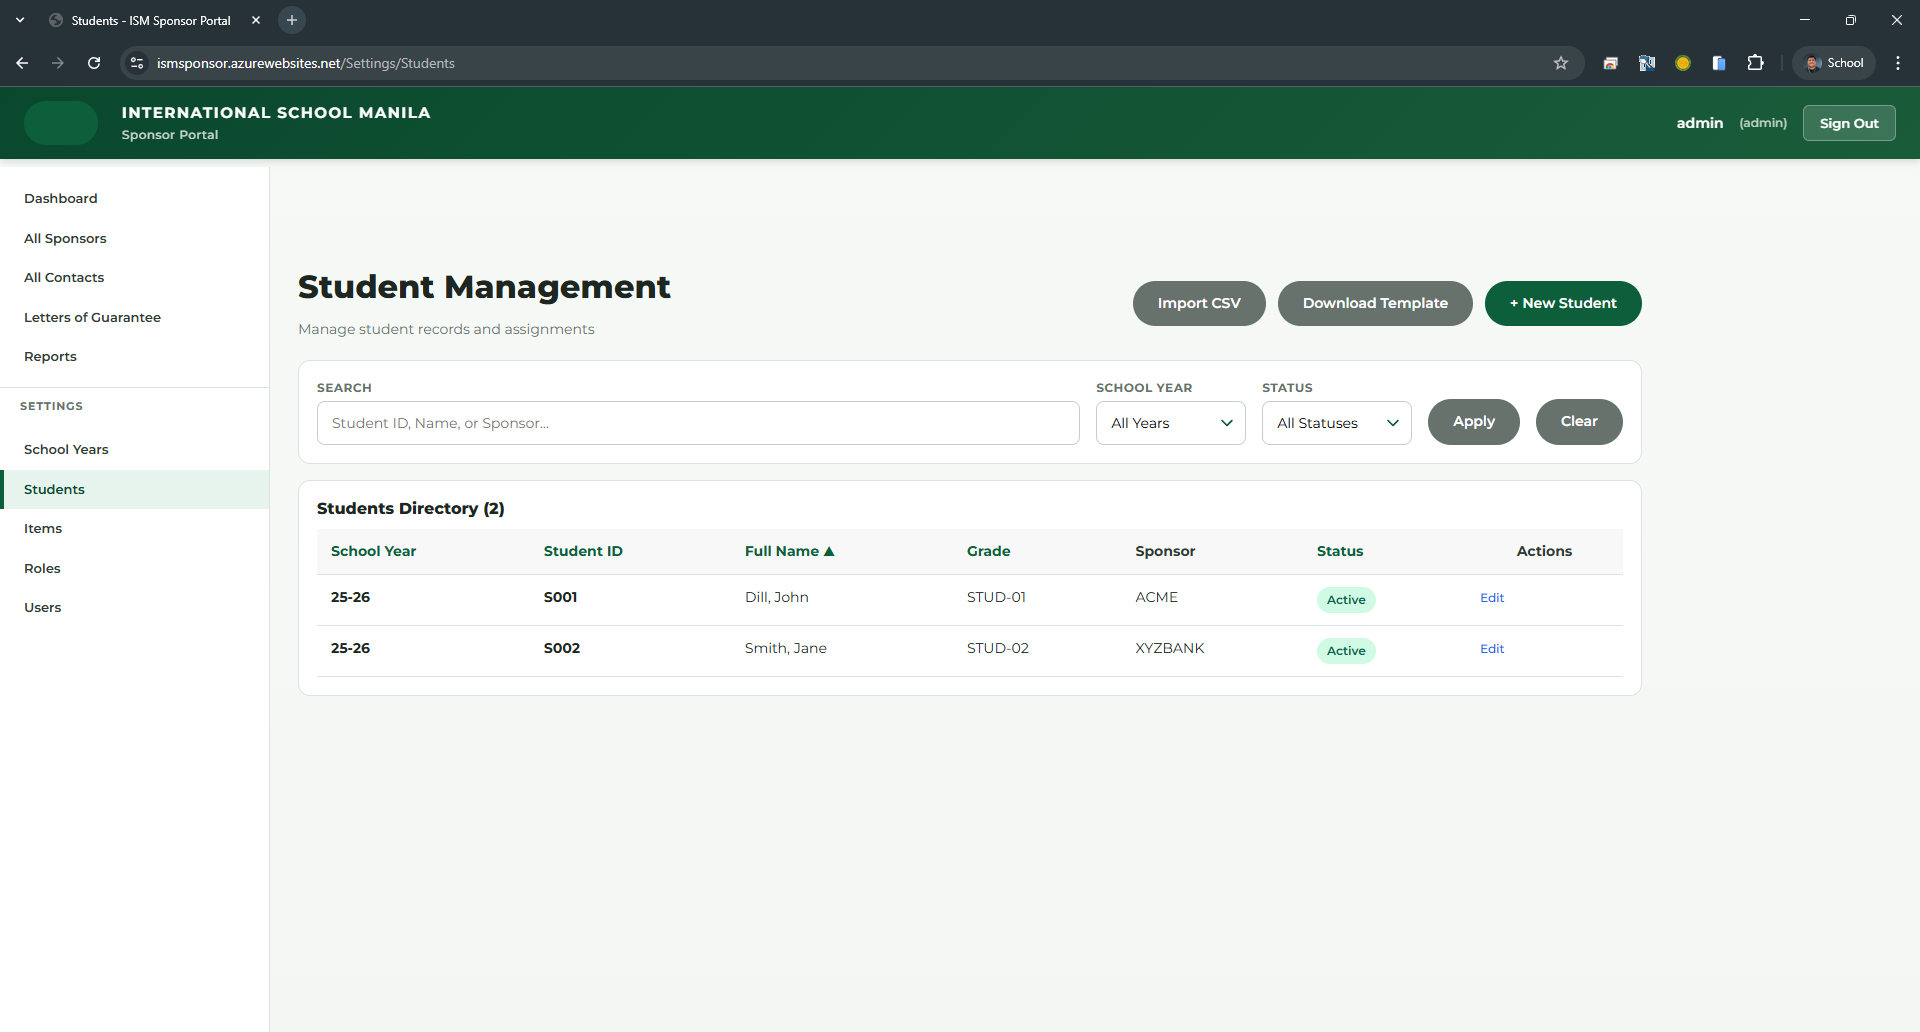
\includegraphics[width=0.90\linewidth]{images/current-interface/admin_students.png}
        \caption{Student Management page}
        \label{fig:current-student-management}
    \end{figure}

    \noindent Figure~\ref{fig:current-student-management} details the Student Management page, where student records can be searched and reviewed by school year, sponsor, and status. The figure is included to show how student references support sponsor assignment and LoG coverage validation.

    \begin{figure}[H]
        \centering
        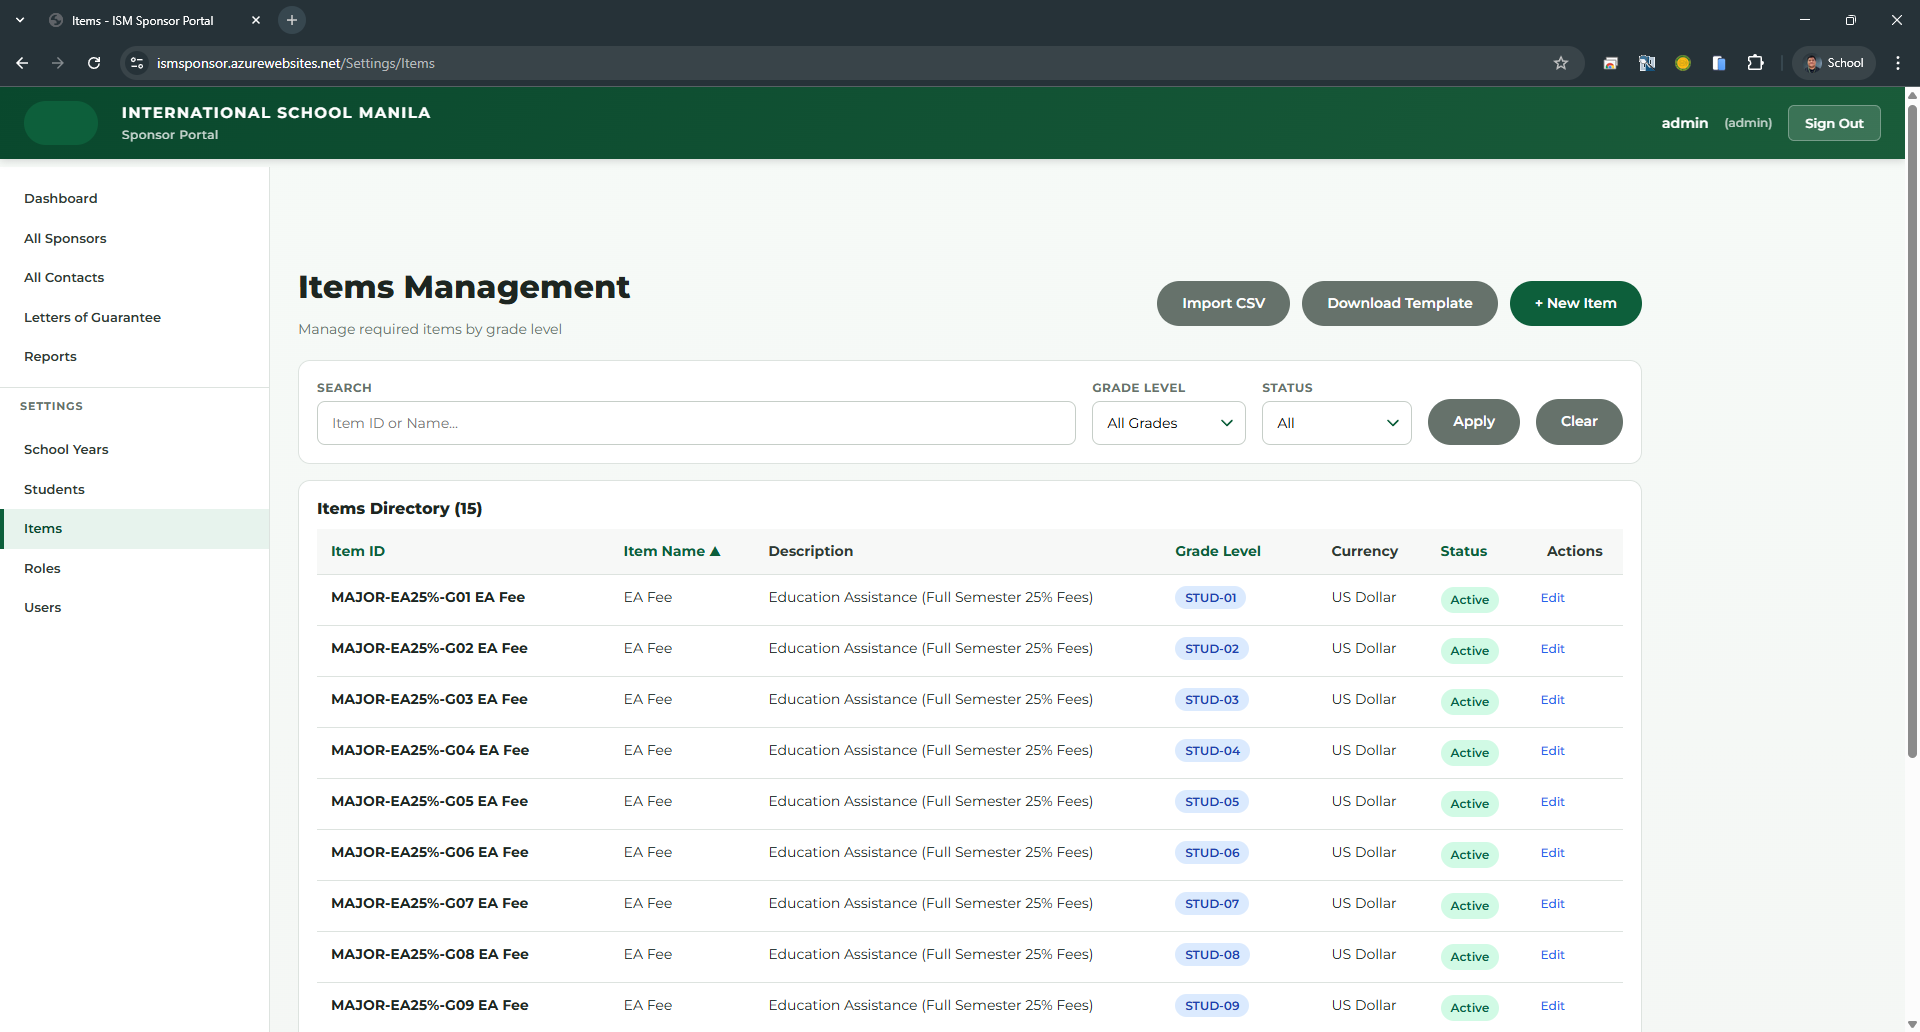
\includegraphics[width=0.90\linewidth]{images/current-interface/admin_items.png}
        \caption{Items Management page}
        \label{fig:current-items-management}
    \end{figure}

    \noindent Figure~\ref{fig:current-items-management} details the Items Management page, which maintains the charge items used in coverage evaluation. The figure is included to show how item-level reference data supports deterministic matching between a charge and the related LoG coverage rule.

    \begin{figure}[H]
        \centering
        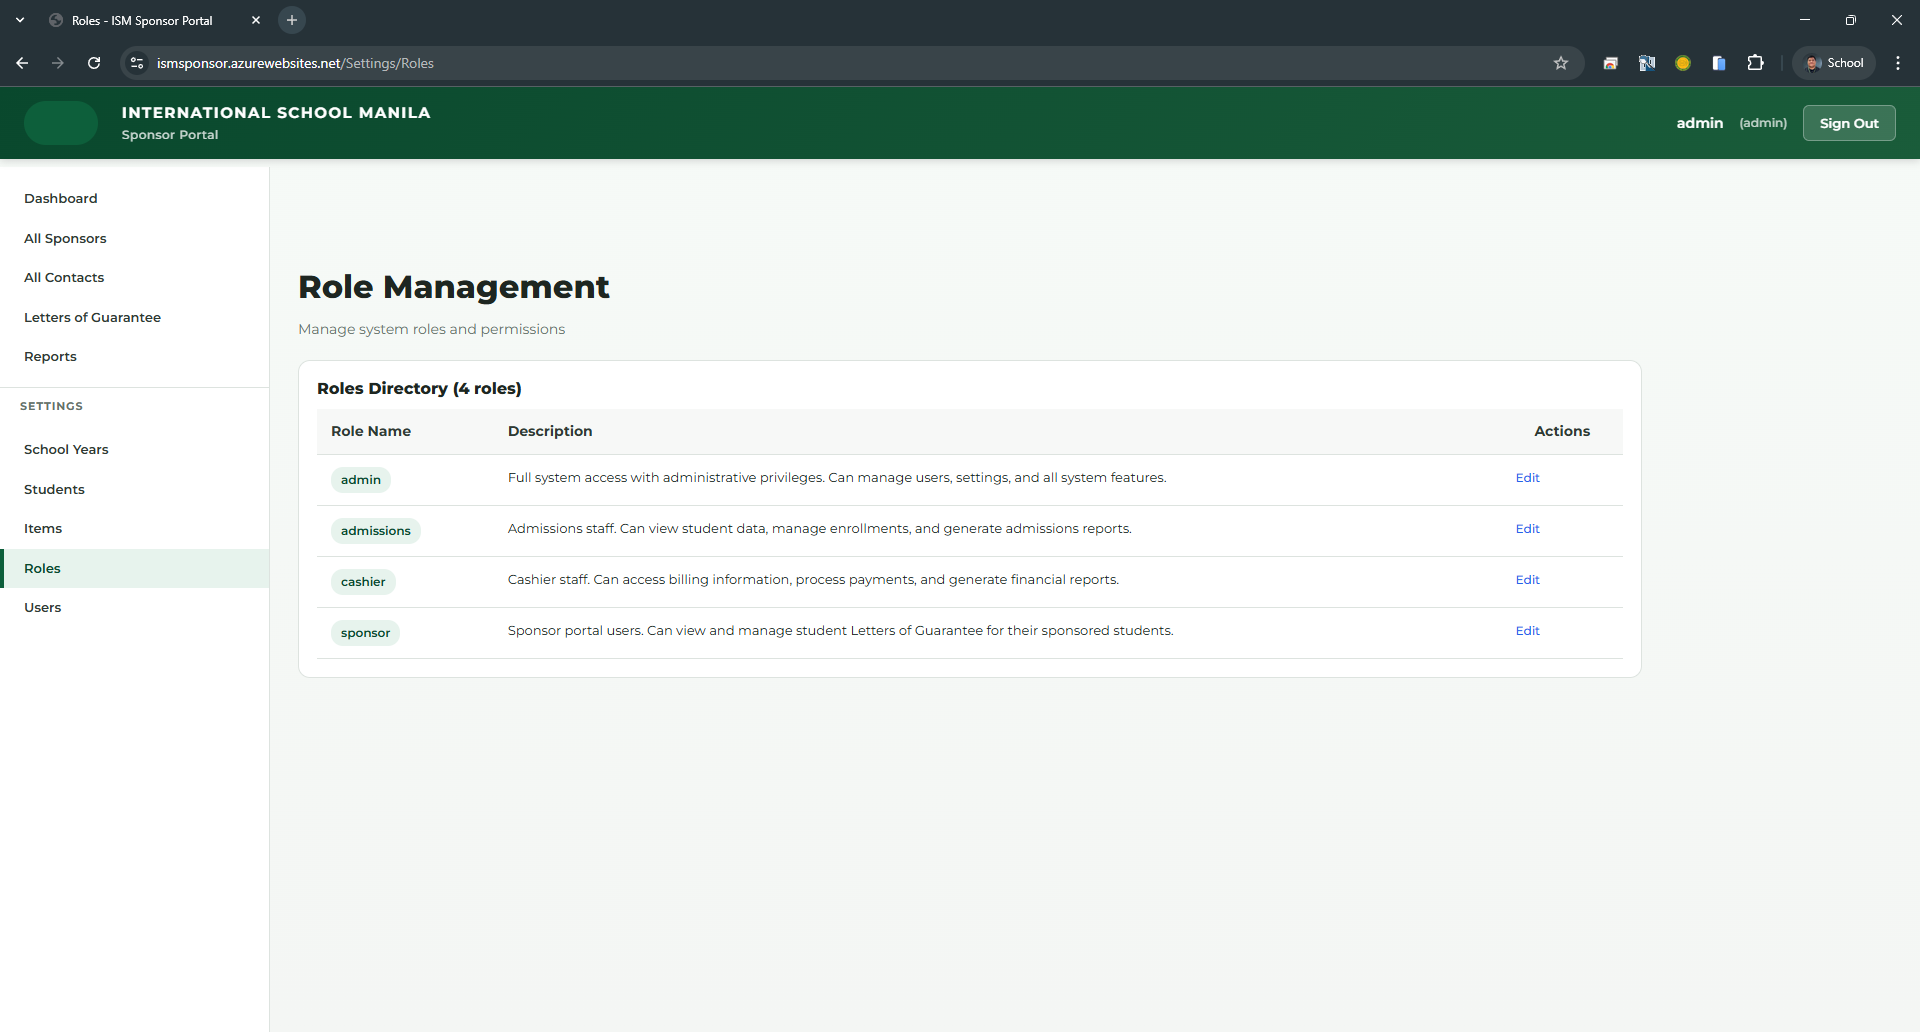
\includegraphics[width=0.90\linewidth]{images/current-interface/admin_roles.png}
        \caption{Role Management page}
        \label{fig:current-role-management}
    \end{figure}

    \noindent Figure~\ref{fig:current-role-management} details the Role Management page, which defines role records used for access control. The figure is included to show how the pilot separates administrative, admissions, cashier, and sponsor permissions.

    \begin{figure}[H]
        \centering
        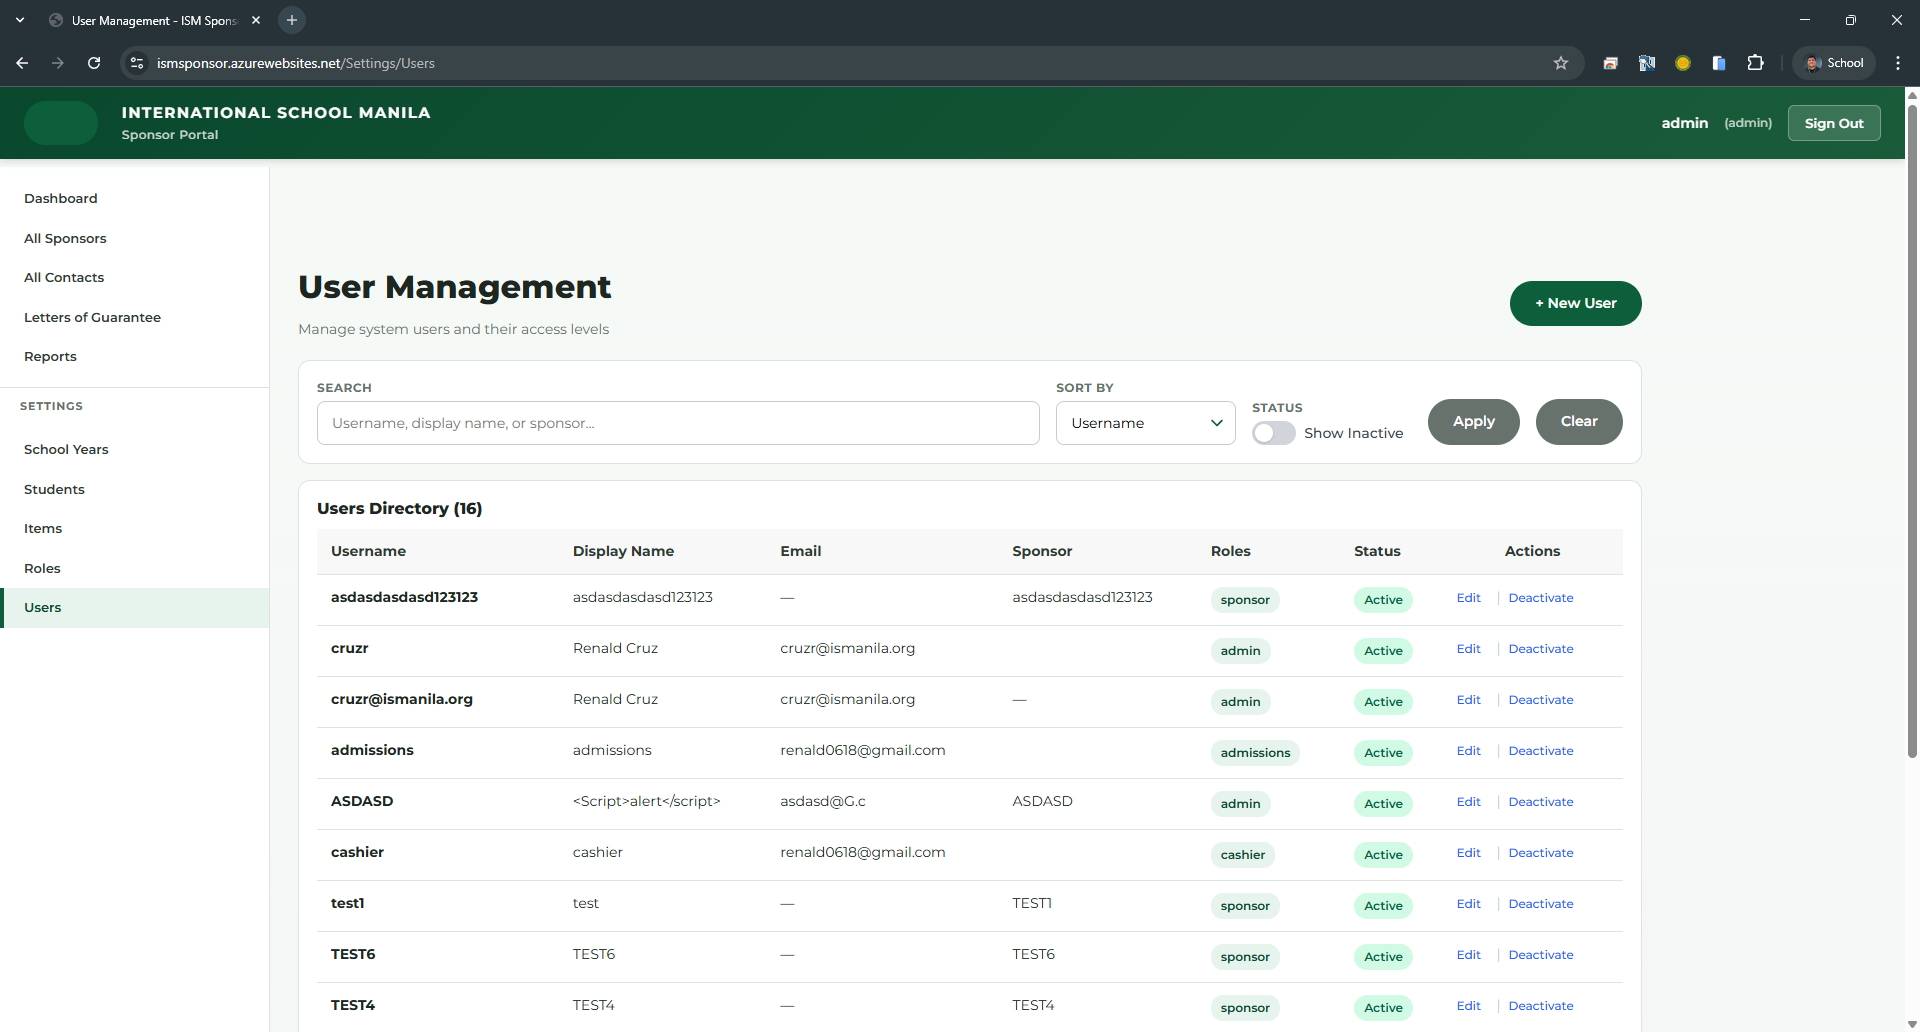
\includegraphics[width=0.90\linewidth]{images/current-interface/admin_users.png}
        \caption{User Management page}
        \label{fig:current-user-management}
    \end{figure}

    \noindent Figure~\ref{fig:current-user-management} details the User Management page, where user accounts, role assignments, and sponsor account links are administered. The figure is included to show how access governance is maintained for both internal users and sponsor-facing accounts.
    \clearpage
